% !TeX document-id = {e7fef4b9-afbc-4e81-94aa-c4847183d047}
% !BIB program = biber
\documentclass[conference, a4paper, 10pt, times]{IEEEtran}
\usepackage{nopageno}

%\usepackage[T1]{fontenc}
\usepackage{amsfonts}
\usepackage{amsmath}
\usepackage{amsthm}
\usepackage{bm}

\usepackage[dvipsnames]{xcolor}
\usepackage{graphicx}
\usepackage{tikz}
\usetikzlibrary{arrows.meta, calc, fit, positioning}

\usepackage{etoolbox}
\usepackage[binary-units, per-mode=symbol]{siunitx}
\robustify\bfseries
\sisetup{detect-all, range-phrase=--, range-units=single, detect-weight=true,detect-inline-weight=math}

\makeatletter
\let\MYcaption\@makecaption
\makeatother

\usepackage[font=footnotesize]{subcaption}

\makeatletter
\let\@makecaption\MYcaption
\makeatother

\usepackage[basic]{complexity}
\usepackage[super,negative]{nth}

\usepackage[british]{babel}
\usepackage{csquotes}

\usepackage{booktabs}
\usepackage[
activate={true,nocompatibility},
final,
tracking=true,
%kerning=true,spacing=true
]{microtype}
\microtypecontext{spacing=nonfrench}

%% Fix indent in new section...
\newcommand{\subparagraph}{}
\usepackage{titlesec}
\titlespacing*{\section}{0pt}{1.5ex}{0.7ex}
\titlespacing*{\subsection}{0pt}{1.5ex}{0.7ex}
\titlespacing*{\paragraph}{0pt}{1.5ex}{0.7ex}
%\titleformat*{\filcenter\scshape}

\usepackage{enumitem}
\setlist[description]{leftmargin=8em,style=nextline}

%bib
\usepackage[style=ieee,maxnames=3,mincitenames=1,maxcitenames=2,maxbibnames=99,
mincrossrefs=99,minxrefs=99,
sortcites,
%backend=bibtex,
uniquelist=false]{biblatex}
\addbibresource{papers-off.bib}
\addbibresource{confs-off.bib}
\addbibresource{books-off.bib}
\addbibresource{rfc.bib}
\addbibresource{misc.bib}

%picky abt et al.
%\usepackage{xpatch}

%\xpatchbibmacro{name:andothers}{%
%	\bibstring{andothers}%
%}{%
%	\bibstring[\emph]{andothers}%
%}{}{}

% emph'd et al. for ieee style
\DefineBibliographyStrings{english}{%
	andothers = {\emph{et al}\adddot}
}
\DeclareFieldFormat[inproceedings]{url}{}
\DeclareFieldFormat[article]{url}{}
\DeclareFieldFormat[inproceedings]{doi}{}
\DeclareFieldFormat[article]{doi}{}
\DeclareFieldFormat[inproceedings]{editor}{}
\DeclareFieldFormat[proceedings]{editor}{}
\DeclareFieldFormat[article]{editor}{}

% Thanks to http://codydunne.blogspot.com/2012/01/suppressing-bibtex-fields-for-specific.html
\AtEveryBibitem{% Clean up the bibtex rather than editing it
	\clearlist{address}
%	\clearfield{date}
%	\clearfield{eprint}
	\clearfield{isbn}
	\clearfield{issn}
	\clearlist{location}
%	\clearfield{month}
	\clearfield{series}
	
	\ifentrytype{book}{}{% Remove publisher and editor except for books
		\clearlist{publisher}
		\clearname{editor}
	}
}

%opening!

\newcommand{\mytitle}{Improving Direct-Control Reinforcement Learning for Network Intrusion Prevention}
%\newcommand{\mytitle}{Per-Host DDoS Mitigation by Direct-Control Reinforcement Learning}

\usepackage{url}
\usepackage{hyperref}
\usepackage[nameinlink]{cleveref}
\newcommand{\crefrangeconjunction}{--}

\hypersetup{
	colorlinks,
	citecolor=black,
	filecolor=black,
	linkcolor=black,
	urlcolor=black,
	pdftitle={\mytitle{}},
%	pdfauthor={Kyle A. Simpson, Simon Rogers, Dimitrios P. Pezaros}
	pdfauthor={Anonymous Giraffe, Anonymous Badger, Anonymous Ibex}
}
\newcommand*{\email}[1]{\href{mailto:#1}{\nolinkurl{#1}} } 

\usepackage{titling}
%\settowidth{\thanksmarkwidth}{*}
%\setlength{\thanksmargin}{-\thanksmarkwidth}
%
%%% Enable /thanks
%\IEEEoverridecommandlockouts
%\makeatletter
%\def\footnoterule{\relax%
%	\kern-5pt
%	\hbox to \columnwidth{\hfill\vrule width 0.5\columnwidth height 0.4pt\hfill}
%	\kern4.6pt}
%\makeatother

% make math easy
\newcommand{\acval}[3]{\ensuremath{\operatorname{\hat{q}}(#1, #2, #3)}}
\newcommand{\wvec}[1]{\ensuremath{\bm{w}_{#1}}}

%thm environments
\newtheorem{thm}{Theorem}
\newtheorem{corr}{Corollary}[thm]

\newcommand{\fakepara}[1]{\noindent\textbf{#1:}}

\makeatletter\let\expandableinput\@@input\makeatother

\makeatletter
\DeclareRobustCommand{\rvdots}{%
	\vbox{
		\baselineskip4\p@\lineskiplimit\z@
		\kern-\p@
		\hbox{.}\hbox{.}\hbox{.}
}}
\makeatother

% Official colours!

\definecolor{uofguniversityblue}{rgb}{0, 0.219608, 0.396078}

\definecolor{uofgheather}{rgb}{0.356863, 0.32549, 0.490196}
\definecolor{uofgaquamarine}{rgb}{0.603922, 0.72549, 0.678431}
\definecolor{uofgslate}{rgb}{0.309804, 0.34902, 0.380392}
\definecolor{uofgrose}{rgb}{0.823529, 0.470588, 0.709804}
\definecolor{uofgmocha}{rgb}{0.709804, 0.564706, 0.47451}

\definecolor{uofglawn}{rgb}{0.517647, 0.741176, 0}
\definecolor{uofgcobalt}{rgb}{0, 0.615686, 0.92549}
\definecolor{uofgturquoise}{rgb}{0, 0.709804, 0.819608}
\definecolor{uofgsunshine}{rgb}{1.0, 0.862745, 0.211765}
\definecolor{uofgpumpkin}{rgb}{1.0, 0.72549, 0.282353}
\definecolor{uofgthistle}{rgb}{0.584314, 0.070588, 0.447059}
\definecolor{uofgpillarbox}{rgb}{0.701961, 0.047059, 0}
\definecolor{uofglavendar}{rgb}{0.356863, 0.301961, 0.580392}

\definecolor{uofgsandstone}{rgb}{0.321569, 0.278431, 0.231373}
\definecolor{uofgforest}{rgb}{0, 0.317647, 0.2}
\definecolor{uofgburgundy}{rgb}{0.490196, 0.133333, 0.223529}
\definecolor{uofgrust}{rgb}{0.603922, 0.227451, 0.023529}

\definecolor{inferno0}{rgb}{0.001462 0.000466 0.013866}
\definecolor{inferno64}{rgb}{0.341500 0.062325 0.429425}
\definecolor{inferno128}{rgb}{0.735683 0.215906 0.330245}
\definecolor{inferno192}{rgb}{0.978422 0.557937 0.034931}
\definecolor{inferno255}{rgb}{0.988362 0.998364 0.644924}

\colorlet{lowac}{inferno128}
\colorlet{midac}{inferno192}
\colorlet{highac}{inferno255}

%-------------------------------------%
%-------------------------------------%

\title{\mytitle{}}
\author{
%	Kyle A.\ Simpson\thanks{This work was supported by the Engineering and Physical Sciences Research Council [grant number EP/M508056/1].},
%	Kyle A.\ Simpson,
%	Simon Rogers,
%	Dimitrios P.\ Pezaros,\\
%	University of Glasgow, Glasgow, Scotland,\\
%	\email{k.simpson.1@research.gla.ac.uk}
Anonymous Giraffe,
Anonymous Badger,
Anonymous Ibex\\
Unnamed Department, Nowhere\\
\email{giraffe.a@unnamed.com}
}

% Remove date, leave no spacing.
\predate{}
\postdate{}
\date{}

\begin{document}

%% If needed, make urls typewritery
%\urlstyle{tt}

\maketitle

\begin{abstract}
Network intrusion detection and prevention systems backed by machine learning (and the autonomous operation they promise) have been long-awaited, but face problems hampering effective deployment.
The detection problem in this domain presents unique difficulties; it is an evolving, non-stationary problem as usage patterns shift and new protocols and applications are introduced, further compounded by burstiness and seasonal variation.

\emph{Reinforcement learning} (RL) may overcome the detection problem for certain classes of anomaly by managing and monitoring \emph{consequences}; an agent's role is to learn to optimise performance criteria (which are always available).
We examine how the paradigm has been applied to the task of \emph{Distributed Denial of Service} (DDoS) attack prevention to date, and present an analysis of suspected edge cases to uncover existing weaknesses in present approaches.
These flaws---poor handling of TCP traffic and high host density at egress points---inspire and direct an exploration of the design space of RL models.
We advance the state-of-the-art of DDoS mitigation using RL by introducing two agent classes designed to act on a per-flow basis, in a protocol-agnostic manner.
This is supported by an in-depth investigation of feature suitability and empirical evaluation.

Our results show the existence of flow features with high predictive power for environments with predominantly TCP or UDP traffic, when such features are used as a basis for feedback-loop-like control.
We show that the new RL agent models can offer a significant increase in goodput of legitimate UDP traffic for many choices of host density, alongside a marked increase in protected TCP traffic at high host density.

\end{abstract}

\section{Introduction}

Network anomaly detection and intrusion detection/prevention are continually evolving problems, compounded by the partial, non-\emph{independent and identically distributed} (IID) view of data at each point in the network.
Attacks and anomalous behaviours evolve, becoming more sophisticated or employing new vectors to harm a network or system's confidentiality, integrity, and availability without being detected \cite{DBLP:journals/comsur/BhuyanBK14}.
These attacks and anomalies have measurable consequences and symptoms which allow a skilled analyst to infer new signatures for detection by misuse-based classifiers, but unseen attacks may only be defended against after-the-fact.
This issue is inherent to \emph{misuse-} or \emph{signature-based} intrusion detectors, and it has been long-hoped that \emph{anomaly-based} detectors would surpass this by making effective use of statistical measures \cite{DBLP:journals/comsur/BhuyanBK14}.

While \emph{machine learning} (ML) approaches seem like a sensible fit for this problem, in \citeyear{DBLP:conf/sp/SommerP10} \citeauthor{DBLP:conf/sp/SommerP10} identified the `failure to launch' of ML-based anomaly detection systems---a distinct lack of real-world system deployments \cite{DBLP:conf/sp/SommerP10}.
To quite a large extent, this remains the case today.
These authors posit that their application is made difficult due to significant operational differences from standard ML tasks, including: the high cost of errors and extraordinarily low tolerance for false positives inherent to network intrusion detection \cite{DBLP:conf/ccs/Axelsson99}; a general lack of recent, openly available (and high-quality) training data; and diversity of network traffic across varying timescales combined with significant burstiness \cite{DBLP:journals/ccr/LelandWTW95}.
Above the aggregate level, the constant deployment of new services and new protocols means that traffic is \emph{non-stationary} and displays an evolving notion of normality.
Learning is made harder still by the challenges encountered when learning from unlabelled (often partial) data.
All of these factors greatly inflate the difficulty of the detection problem.

%?? Make it clearer here what problem I specifically want to solve: principally a particular class of DDoS attacks; volume-based DDoS attacks. Amplification attacks are just a specialisation, this can be made more obvious. I think I need to be clearer about the \emph{intended deployment environment} of service hosts (i.e., not ISPs).

For certain classes of problem e.g., volume-based \emph{distributed denial of service} (DDoS) attacks, \emph{reinforcement learning} (RL) offers another perspective.
%?? Unclear explanation of RL here?
RL agents operate by following a \emph{policy} to interact with or control a system, while at the same time using observed performance metrics and deliberate exploration to dynamically improve this policy.
In this way the role of a RL agent differs from that of a standard classifier, adaptively reacting to threats by assuming the role of a feedback loop for network optimisation, typically to safeguard service guarantees.
In a sense, this allows us to ``overcome'' some of the difficulties of the detection problem by monitoring \emph{performance characteristics and consequences} in real-time; by looking for (and controlling) the effect rather than the cause.
Long-term, we expect that the value of RL-based defence systems will be to augment what existing misuse-based solutions can provide, by automatically alerting, recording and controlling what are believed to be illegal system states.
The goal of this work is much less general; we aim to prevent volume-based DDoS attacks with the aid of RL-based techniques (an important goal in its own right), while bringing to light the flexibility and applicability of these techniques in the security domain.
%Whether it takes direct control of the network, or is used indirectly to optimise a key part of another system, more powerful `deep' RL techniques (and well-founded action spaces) aren't yet well explored for network IDS/IPS.
%These range from more modern training algorithms \cite{DBLP:journals/corr/SchulmanWDRK17, DBLP:conf/icml/SchulmanLAJM15}, to evolutionary strategies \cite{DBLP:journals/corr/SalimansHCS17, DBLP:journals/corr/abs-1802-08842}, hierarchical action composition \cite{DBLP:journals/corr/abs-1710-09767}, and competitive multi-agent learning \cite{DBLP:journals/corr/abs-1710-03748}.

To date, there have been few applications of this class of algorithms towards intrusion detection and prevention which make use of their full potential for online control, rather than using them as the basis for a classifier.
We aim to take steps to redress this and establish their proper capabilities, beyond simple ``blind application''.
%?? Expand as required
What approaches do exist are aimed towards the task of adaptive online DDoS mitigation, and rely upon learning control of probabilistic packet drop.
%?? THAT IS A MAJOR CONTRIB, MENTION IT EVERYWHERE YOU CAN

%?? Discuss the most important conclusions before the outline.
We find that the existing work for this task fails to account for congestion-aware traffic (i.e., TCP) and deployment environments with high host density per egress point, achieving poor results due to an overly coarse view of the network.
The approach we identify to remedy this is to make throttling decisions on a per-source basis, and we present the engineering decisions this mandates: updating RL agents from multiple traces per timestep, timed random sequential action computation and a supporting \emph{software-defined network} (SDN) architecture.
In tandem with the development and evaluation of an effective state-space and model, we provide the design of a second model inspired by past work on algorithmic DDoS prevention, as an example of the integration of domain-specific knowledge.
Our introduction of per-source decisions improves substantially upon the state-of-the-art, and we show that our second model achieves excellent performance for high host density.
Crucially, both models remain protocol- and content-agnostic to offer future-proofing against the rollout of future protocols like QUIC \cite{DBLP:conf/sigcomm/LangleyRWVKZYKS17}.
%?? Also algorithmic enhancements such as multiple actions per timestep, 
%?? PROTOCOL-AGNOSTIC -- HOW WILL THESE THINGS COPE WITH QUIC ET AL.?!?!
Briefly, this paper contributes:
\begin{itemize}
%	\item A DDoS mitigation system based on direct-control reinforcement learning, designed for deployment in real-world software-defined networks (\cref{sec:environment-and-rl-algorithm,sec:acting-on-individual-sources}).
	\item Important weaknesses and flaws in the past design and evaluation of similar techniques \cite{DBLP:journals/eaai/MalialisK15}. We offer a deconstruction and empirical study on their formulation, flaws, and risk factors concerning different traffic distributions---in addition, we demonstrate modifications enabling deployment in real-world software-defined networks (\cref{sec:performance-in-an-emulated-environment}).
	\item A reactive simulation of web-server traffic, designed to test system characteristics that packet trace playback fails to capture (\cref{sec:a-new-normal}).
	\item An in-depth investigation into suitable features for an automatic DDoS mitigation system, with qualitative and quantitative justification (\cref{sec:rethinking-the-state-space}).
	\item Two source-level granularity approaches to RL-driven DDoS prevention (\emph{Marl++}, \emph{SPF}), improving upon past aggregate-based models (\cref{sec:acting-on-individual-sources}), alongside an empirical evaluation (\cref{sec:the-results-of-doing-so}) and discussion of security concerns and real-world deployment (\cref{sec:discussion}).
\end{itemize}

\section{Background and Threat Model}
%?? Introduce RL, related definitions etc.

\subsection{Distributed Denial of Service}
%?? DDoS attack variants (leading into characteristics, supporting features). Amplification (UDP \cite{DBLP:conf/ndss/Rossow14}, TCP \cite{DBLP:conf/uss/KuhrerHRH14}), Transit-link (Crossfire \cite{DBLP:conf/sp/KangLG13}, Coremelt \cite{DBLP:conf/esorics/StuderP09}). Mirai botnet's involvement \cite{DBLP:conf/uss/AntonakakisABBB17}.

%?? Explain amplification attack, maybe transit-link?

\emph{Distributed denial of service} (DDoS) attacks are concentrated efforts by many hosts to reduce the availability of a service, typically to inflict financial harm or as an act of vandalism.
Attackers achieve this either by exploiting peculiarities of operating system or application behaviour (e.g., \emph{SYN flooding attacks}), or overwhelming their target through sheer volume of requests or inbound packets (\emph{flooding-based attacks}).
Hosts often participate unwillingly, typically having been recruited into a \emph{botnet} by malware infection to be orchestrated from elsewhere \cite{DBLP:conf/uss/AntonakakisABBB17}.

Although there are variations of each class of attack, flooding attacks are the most relevant to our work.
\emph{Amplification attacks} exploit the presence of services who eagerly send large replies in response to small requests, where UDP-based services like DNS and NTP are most exploitable \cite{DBLP:conf/ndss/Rossow14, DBLP:conf/uss/KuhrerHRH14}.
Malicious hosts send many small requests, spoofed to appear as though they originated from the victim, causing many large replies to be sent to the intended target---significantly increasing a botnet's throughput while masking the identity of each participant.
\emph{Transit-link/link-flooding attacks} have been the subject of recent attention, wherein malicious traffic is forwarded across core links needed to reach a target (but not to the target itself) \cite{DBLP:conf/sp/KangLG13, DBLP:conf/esorics/StuderP09}.

?? EXPAND

\subsection{Reinforcement Learning}\label{sec:reinforcement-learning}
\emph{Reinforcement learning} (RL) is a variant of machine learning principally concerned with training an agent to choose an optimal sequence of actions in the pursuit of a given task \cite{RL2E}.
We assume the agent has a certain amount of knowledge whenever a decision must be made: at any point in time $t$, it knows which \emph{state} it is in ($S_t \in \mathcal{S}$), the set of \emph{actions} which are available to it ($\operatorname{A}(S_t) \subseteq \mathcal{A}$) and, if available, a numeric \emph{reward} obtained from the last action chosen ($R_t \in \mathbb{R}, A_{t-1} \in \operatorname{A}(S_{t-1})$).
This model of system interaction is best described as a \emph{Markov Decision Process} (MDP).
RL methods combine this information with a current \emph{policy} $\pi$ to determine which action should be taken: such a choice need not be optimal if an agent needs to further explore some region of the state space.
The policy is then further refined by updating value estimates for state-action pairs or via policy gradient methods, meaning that RL-based approaches learn adaptively and online if reward functions are available in the environment they are deployed in.
In practice, this means that agents are able to automatically adapt to evolving problems without operator intervention or a new, custom-built training corpus.

From any point in a sequence of decisions, we may describe the sum of rewards yet to come as the \emph{discounted return}, $G_t = R_{t+1} + \gamma R_{t+2} + \gamma^2 R_{t+3} + \ldots$, choosing the discount factor $\gamma \in [0,1)$ to determine how crucial future rewards are vis-\`{a}-vis the current state.
Formally, an agent's goal is to choose actions which maximise the \emph{expected discounted return} $\operatorname{\mathbb{E}_{\pi}}[G_t]$.

%?? Include some details of function approximation in the formalisation? I.e. tile coding, stability and convergence guarantees...

There is immense variation in \emph{how} policies and/or values may be learned, reliant upon the learning environment, problem and required convergence guarantees.
In particular, we shall focus on methods which choose actions according to their value estimates from the current state: let $\operatorname{q}(s, a) \in \mathbb{R}$ denote the estimate of action $a$'s value if it were to be taken in state $s$.
%?? Revisit the maths here, d, dim A, s...
Exact (tabular) representations require that we store a value estimate for each action in every state---if state is real-valued or high-dimensional, then computation and storage quickly become infeasible.
To cope with a continuous state and/or action space, one valuable technique is to employ linear function approximation backed by \emph{tile coding} \cite[pp.\ \numrange{217}{221}]{RL2E}.

\begin{figure}
	\centering
	\begin{subfigure}{0.4\linewidth}
		\resizebox{\linewidth}{!}{
		\begin{tikzpicture}
		\node at (0,0.3){$s = \begin{pmatrix}
			0.7 \\
			0.3
			\end{pmatrix}$};
		\node at (0,-1) {$\bm{x}(s,\cdot) = \begin{Bmatrix}
			T_{1,9}, \\
			T_{2,5}, \\
			T_{\mathit{bias}}
			\end{Bmatrix}$};
		
		\node at (2.5,-0.5) {
			\begin{tikzpicture}
			\draw[step=0.5cm,color=uofgcobalt,opacity=0.7,shift={(0,0)},label=above:{Tiling 0}] (-0.5,-0.5) grid (1,1);
			\fill[uofgcobalt,opacity=0.5] (0.5,-0.5) rectangle (1,0);
			\node[color=uofgcobalt] at (0,1.1) {\footnotesize Tiling 1};
			
			\draw[step=0.5cm,color=uofgpumpkin,opacity=0.7,shift={(0.25,-0.25)},label=above:{Tiling 1}] (-0.5,-0.5) grid (1,1);
			\fill[uofgpumpkin,opacity=0.5,shift={(0.25,-0.25)}] (0,0) rectangle (0.5,0.5);
			\node[color=uofgpumpkin] at (0.25,-0.95) {\footnotesize Tiling 2};
			
			\node[circle, black, draw,
			fill, radius=0.5pt, inner sep=0pt,minimum size=1.5pt, label=above:{$s$}] at (0.625,-0.125) {};
%			\filldraw (0.625,-0.125) circle[radius=1.5pt,label=above:{$s$}];

			\draw[->] (-0.25,-0.5)--(-0.25,0.85);
			\draw[->] (-0.25,-0.5)--(1.1,-0.5);
			
			\node at (1,-0.7) {\footnotesize 1};
			\node at (-0.4,0.75) {\footnotesize 1};
			\node at (-0.35,-0.6) {\footnotesize 0};
			\end{tikzpicture}
		};
		
		\end{tikzpicture}
		}
		\caption{Tile Coding\label{fig:tilecode-code}}
	\end{subfigure}%
	\begin{subfigure}{0.4\linewidth}
		\resizebox{\linewidth}{!}{
		\begin{tikzpicture}
		% Top half
		\def\topacs{
			{-0.3,-0.5,-0.1,0.8},
			{0.1,0.1,-0.2,0.3},
			{0.3,0.4,0.2,-0.4}%
		}
	
		\foreach \line [count=\y] in \topacs {
			\foreach \pix [count=\x] in \line {
				\ifthenelse{\lengthtest{\pix pt < 0 pt}}{
					\pgfmathtruncatemacro\lambda{(\pix+1)*100}
					\draw[shift={(-0.7,0)},fill=midac!\lambda!lowac] (0.7*\x,-0.35*\y) rectangle +(0.7,0.35);
				}{
					\pgfmathtruncatemacro\lambda{\pix*100}
					\draw[shift={(-0.7,0)},fill=highac!\lambda!midac] (0.7*\x,-0.35*\y) rectangle +(0.7,0.35);
				}
				\node[shift={(-0.35,0.175)}] at (0.7*\x,-0.35*\y) {\footnotesize \pix};
			}
		}
	
		\draw[xstep=0.7cm,ystep=0.35cm,shift={(0,0)}] (0,-1.06) grid (2.8,0);
		\node[label=left:{$T_{1,9}$},shift={(0,-0.125)}] at (0,0) {}; 
		\node[label=left:{$T_{2,5}$},shift={(0,-0.125)}] at (0,-0.375) {}; 
		\node[label=left:{$T_{\mathit{bias}}$},shift={(0,-0.125)}] at (0,-0.75) {};
		
		% bottom half
		\def\botacs{
			{0.1,0.0,-0.1,0.7}%
		}
	
		\foreach \line [count=\y] in \botacs {
			\foreach \pix [count=\x] in \line {
				\ifthenelse{\lengthtest{\pix pt < 0 pt}}{
					\pgfmathtruncatemacro\lambda{(\pix+1)*100}
					\draw[shift={(-0.7,-1.275)},fill=midac!\lambda!lowac] (0.7*\x,-0.35*\y) rectangle +(0.7,0.35);
				}{
					\pgfmathtruncatemacro\lambda{\pix*100}
					\draw[shift={(-0.7,-1.275)},fill=highac!\lambda!midac] (0.7*\x,-0.35*\y) rectangle +(0.7,0.35);
				}
				\node[shift={(-0.35,-1.1)}] at (0.7*\x,-0.35*\y) {\footnotesize \pix};
			}
		}
	
		\draw[xstep=0.7cm,ystep=0.35cm,shift={(0,-1.275)}] (0,-0.35) grid (2.8,0);
		\node[label=left:{$\mathit{Total}$},shift={(0,-0.175)}] at (0,-1.275) {};
		
		\draw [->] (2.45, -1.9) -- (2.45, -1.65);
		\end{tikzpicture}
		}
		\caption{\centering Value Estimation and Action Selection\label{fig:tilecode-select}}
	\end{subfigure}
	
	\caption{
		An example of tile coding for 2-dimensional state and 4 actions, using 2 tilings, 3 tiles per dimension, and a bias tile.
		All components of $s$ are clamped to the range $[0,1]$.
		For simplicity, we denote $\bm{x}(s,\cdot)$ as a list of indices and represent the values of all actions at each tile with a vector.
		(a) The state $s$ activates the bias tile and exactly one tile in each tiling.
		(b) The action values of active tiles are summed to produce the current value estimate for each action available in $s$---for this state, local knowledge ensures that action 4 is chosen by the greedy policy despite typically being a poor choice elsewhere.
		\label{fig:tilecode}
	}
\end{figure}

Tile coding is a form of feature representation which converts a state-action pair into a sparse boolean feature vector $\operatorname{\mathbf{x}}(s, a)$ by subdividing a $d$-dimensional subset of the space into a number of overlapping grids with an optional bias component.
Each tile corresponds to an entry of $\operatorname{\mathbf{x}}(s, a)$ which is set to 1 if the state-action pair lies within it.
\Cref{fig:tilecode-code} demonstrates the process for a 2-dimensional state space, and that the numbers of tilings and tiles per dimension control feature resolution and generalisation.
Moreover, to capture combinatorial effects or create multi-scale representation we may combine codings by concatenating individual feature vectors.
We may then approximate an action's value with respect to a policy parameter vector $\wvec{}$, defining some $\acval{s}{a}{\wvec{}} \approx \operatorname{q}(s, a)$:
\begin{equation}
%	\begin{gather}
\acval{s}{a}{\wvec{}} = \wvec{}^{\top} \operatorname{\mathbf{x}}(s, a)
%	\end{gather}
\label{eqn:lin-approx}
\end{equation}
As each component of $\wvec{}$ is the value estimate of the corresponding tile, learning an effective policy is equivalent to learning $\wvec{}$.
Given a learning rate $\alpha \in \mathbb{R}$ and initialising $\wvec{0}=\bm{0}$, we may continually update $\wvec{t}$ using the \emph{1-step semi-gradient Sarsa} algorithm \cite[pp.\ \numrange{243}{244}]{RL2E}:
\begin{subequations}
	\begin{gather}
	\delta_t = R_{t+1} + \gamma \acval{S_{t+1}}{A_{t+1}}{\wvec{t}} - \acval{S_t}{A_t}{\wvec{t}},\\
	\bm{w}_{t+1} = \bm{w}_{t} + \alpha \delta_t \nabla{\acval{S_t}{A_t}{\wvec{t}}},
	\end{gather}%
	\label{eqn:sg-sarsa}%
	where $\delta_t$ is known as the \emph{temporal-difference} (TD) error, and the vector gradient $\nabla$ is taken with respect to $\wvec{}$.
\end{subequations}

Computing the approximate value of every action available in the current state forms the basis of a policy.
Actions with maximal value can be chosen each time (the \emph{greedy} policy), we might modify this by taking random actions with probability $\epsilon$ to encourage early exploration (the \emph{$\epsilon$-greedy policy}), or we might use some other mechanism.
\Cref{fig:tilecode-select} extends the prior working example to show how the value of each action is computed (and which action would be chosen by a greedy policy), combining a global estimate ($T_{\mathit{bias}}$) with knowledge particular to each state.

\begin{figure}
	\centering
	\resizebox{0.5\linewidth}{!}{
		\begin{tikzpicture}		
		% Top half
		\def\startacs{
			{0.8},
			{0.3},
			{-0.4}%
		}
		
		\foreach \line [count=\y] in \startacs {
			\foreach \pix [count=\x] in \line {
				\ifthenelse{\lengthtest{\pix pt < 0 pt}}{
					\pgfmathtruncatemacro\lambda{(\pix+1)*100}
					\draw[shift={(-0.7,0)},fill=midac!\lambda!lowac] (0.7*\x,-0.35*\y) rectangle +(0.7,0.35);
				}{
					\pgfmathtruncatemacro\lambda{\pix*100}
					\draw[shift={(-0.7,0)},fill=highac!\lambda!midac] (0.7*\x,-0.35*\y) rectangle +(0.7,0.35);
				}
				\node[shift={(-0.35,0.175)}] at (0.7*\x,-0.35*\y) {\footnotesize \pix};
			}
		}
		
		\draw[xstep=0.7cm,ystep=0.35cm,shift={(0,0)}] (0,-1.06) grid (0.7,0);
		\node[label=left:{$T_{1,9}$},shift={(0,-0.125)}] at (0,0) {}; 
		\node[label=left:{$T_{2,5}$},shift={(0,-0.125)}] at (0,-0.375) {}; 
		\node[label=left:{$T_{\mathit{bias}}$},shift={(0,-0.125)}] at (0,-0.75) {};
		\node[label=below:{\footnotesize Action 4},shift={(0.35,-0.125)}] at (0,-0.75) {};
		\node[label=above:{\footnotesize $\wvec{t}$},shift={(0.35,-0.125)}] at (0,0) {};
		
		\def\finalacs{
			{0.7},
			{0.2},
			{-0.5}%
		}
	
		\foreach \line [count=\y] in \finalacs {
			\foreach \pix [count=\x] in \line {
				\ifthenelse{\lengthtest{\pix pt < 0 pt}}{
					\pgfmathtruncatemacro\lambda{(\pix+1)*100}
					\draw[shift={(2-0.7,0)},fill=midac!\lambda!lowac] (0.7*\x,-0.35*\y) rectangle +(0.7,0.35);
				}{
					\pgfmathtruncatemacro\lambda{\pix*100}
					\draw[shift={(2-0.7,0)},fill=highac!\lambda!midac] (0.7*\x,-0.35*\y) rectangle +(0.7,0.35);
				}
				\node[shift={(2-0.35,0.175)}] at (0.7*\x,-0.35*\y) {\footnotesize \pix};
			}
		}
		
		\draw[xstep=0.7cm,ystep=0.35cm,shift={(2,0)}] (0,-1.06) grid +(0.7,1.06);
		\node[label=below:{\footnotesize Action 4},shift={(2.35,-0.125)}] at (0,-0.75) {};
		\node[label=above:{\footnotesize $\wvec{t+1}$},shift={(0.35,-0.125)}] at (2,0) {};
		
		\draw[->] (0.9,-0.5) -- node[above] {$+ \alpha \delta_t$} (1.8,-0.5);
		\end{tikzpicture}
	}

\caption{
	The update step for \cref{fig:tilecode}, given an observed TD error $\delta_t=-0.2$ (indicating a lower observed reward than the expected long-term value of \num{0.7}) and $\alpha=0.5$.
	Action 4's value is thus reduced in the tiles associated with state $s$, but remains the most likely choice; the negative $\delta_t$ may have arisen from noise in the reward signal.
	For illustrative purposes, we choose an unrealistically high $\alpha$ (typically, $\alpha\le0.05$ is a more reasonable choice).
	\label{fig:tilecode-update}
}
\end{figure}

This combination of algorithm and coding strategy is well-optimised, if actions are discrete; this allows a particularly efficient (vectorised) implementation of the policy and update rules by storing a vector of action values for each tile.
Action values for any state are then obtained by summation of the weight vectors from all activated tiles---taking $|\mathcal{A}|(n_{\mathit{tilings}}-1)$ floating point additions per decision.
Observing that $\nabla{\acval{s}{a}{\wvec{}}} = \operatorname{\mathbf{x}}(s, a)$, further optimisations arise by considering that a tile-coded feature vector is a binary vector of constant Hamming weight (and so is amenable to representation as an array of indices, $s_{\mathit{list}}$).
This means that we need only perform $n_{\mathit{tilings}} + 2$ additions and \num{2} multiplications per model update:
\begin{equation}
\bm{w}_{t+1}[i][\operatorname{index}(A_t)] = \bm{w}_{t}[i][\operatorname{index}(A_t)] + \alpha \delta_t, \forall i \in s_{\mathit{list}}.
\label{eqn:sg-sarsa-opt}
\end{equation}
\Cref{fig:tilecode-update} shows how this applies to our prior example.
If desired we may define a state-space with an arbitrary number of tiles per dimension (higher-resolution, lower generalisation), yet having constant-size state vectors and constant action computation cost ($\mathcal{O}(n_{\mathit{tilings}})$).
Beyond this, we need not store action values for tiles which have not yet been visited, conserving memory.

%?? Is this \emph{actually} just sarsa? We're using fn approx (of course), but this is fraught with its own difficulties. Is it strictly speaking correct to describe it as Sarsa at this point? It's, at the very least, 1-step semi-gradient Sarsa given that it is clearly on-policy w/ fn approx...

%\subsection{Intrusion Detection}
%Probably want to talk about NIDS/IPS,
%?? Discuss mininet? Networking terms? SDN stuff?

\subsection{Motivation}\label{sec:motivation}
%?? What makes RL a suitable method for network anomaly detection, what features are most relevant?
%?? Point I was thinking of: feedback-loop-like model allows monitoring \emph{after} an action is taken to (in theory) allow forgiveness of mistakenly punished flows. This does hinge on taking a flow-by-flow look at the state space, but if we can combine knowledge of current state (duh!), the last action taken (i.e. an indicator of our previous assessment [such as high pdrop $\implies$ bad]) then perhaps a flow which falls off identically to a legit flow can be rescued.
Moving beyond the overt benefits of choosing RL-based defences for coping with non-stationary problems, we believe that there are concrete reasons for their use here.
We have seen that for other domains in particular, misclassification is a serious problem, which can introduce \emph{collateral damage} in the context of DDoS prevention.
In theory, the feedback-loop-like model allows us to monitor flows \emph{after} an action is taken to allow forgiveness of mistakenly punished flows.
This does rely upon the ability to take a flow-by-flow view of the state space, but if we can combine knowledge of current state with the last applied action, then perhaps a flow which falls off identically to a legitimate flow can be rescued.

%Which features might be best suited to this problem?
%?? Relevant features: aggregate network state (load at various points [this has been done, of course]), flow-specific measurements (upload/download ratio when bandwidth above threshold \cite{DBLP:conf/ndss/Rossow14}, packet inter-arrival times, etc.)
Other studies suggest that there are particularly useful features which make the task of online DDoS flow identification feasible.
Aggregate network load observed at various locations suggests the overall health of a network \cite{DBLP:journals/eaai/MalialisK15}, and the ratio of correspondence between pair flows can suggest asymmetry and in many cases illegitimacy \cite{DBLP:conf/ndss/Rossow14}.
Generic volume-based statistics (counts, counts per duration, average packet sizes) have seen effectiveness in such as $k$-nearest neighbours classifiers trained to detect DDoS attacks in progress \cite{DBLP:conf/dsn/LeeKSPY17}.
Most importantly, there is evidence showing behavioural changes in response to bandwidth expansion \cite{DBLP:conf/ndss/KangGS16}, suggesting similar artefacts might arise after throttling, packet drop, or other interference.
%?? If we assume amplification attacks, we know it won't be `random' source IPs (since it's mostly-legit servers who think that they're doing a good job by replying)
%?? If we assume amplification attacks, we know it won't be `random' source IPs (since it's mostly-legit servers who think that they're doing a good job by replying)

%\section{A Plan, of Sorts}
%
%\begin{enumerate}
%	\item The main case for contribution in what I have so far:
%	\begin{itemize}
%		\item Past work reliant on unrealistic network models: tcp-like behaviour (and its effects on collateral damage) not captured, disjoint ranges of traffic distribution (no benign heavy-hitters), ISP-like topology.
%		\item I offer more realistic network emulation environment, better treatment of protocol/traffic characteristics.
%	\end{itemize}
%	\item Forthcoming: rethinking state/action spaces to operate at a finer level of granularity. New network model (live tcp back-and-forth), allows us to test collateral damage assumptions in a more realistic manner (and show clear case for moving beyond work of malialis and kudenko)
%\end{enumerate}

\subsection{Threat Model}

%?? The fine folks at most security conferences will want to see one. I suppose it serves its purpose by delineating what an attacker can/cannot do.

%?? Oultine attacker's goals, particularly wrt SPIFFY.
%?? They want to impact fair-share bandwidth allocation to flows (minimise), they have no worry about being unmasked (there are many available reflectors, which don't need to be bought etc...) [cite the rossow papers about amplification hell].
An attacker's goal is to minimise the fair-share bandwidth allocation that a server can give to any host which connects to it, and they are expected to act rationally in its pursuit.
Threat actors are external and act intentionally, aren't expected to be classified as an \emph{advanced persistent threat}, and likely range from hacktivists to moderately funded adversaries.
We assume that attacks will be bandwidth-based DDoS attacks with the structure of an \emph{amplification attack}, and that traffic aggregates at the target (unlike in a transit-link attack).
?? VERIFY AND RESEARCH THAT: REVIEWER 1 BELIEVES OTHERWISE.
The addresses of the set of unwitting reflector nodes are visible to the target, though any bots taking part in an attack or the machines those bots such attacks are not revealed to the target without communication/collaboration with \nth{3} party organisations such as upstream ISPs.
The discovery of any reflector by some defence system does have a cost to the attacker---there is a particularly large (yet finite) supply of viable reflector nodes \cite{DBLP:conf/ndss/Rossow14}, but the constraints that each has a large upstream bandwidth and support for high-amplification-factor protocols narrow this pool.

We do not assume that an attacker has white-box access to the parameters underlying an agent's policy, or that they will attempt to intelligently modify flow/system state to indirectly control an agent \cite{DBLP:conf/eurosp/PapernotMJFCS16, DBLP:conf/eurosp/PapernotMSW18, DBLP:journals/corr/HuangPGDA17, DBLP:conf/sp/Carlini017}.
While they may be able to perform some degree of reverse engineering by observing the health of their own legitimate canary flows, ``stealing'' the policy through observation \cite{DBLP:conf/uss/TramerZJRR16}, investigating whether perturbations would persist in a medium as volatile as network traffic statistics falls outside of the scope of this work.
The same observation extends to the possibility of poisoning attacks \cite{DBLP:journals/jmlr/KloftL10, DBLP:conf/acsac/ShenTS16}; to the best of our knowledge, no studies have been undertaken surrounding the mis-training of RL agents.
These are APT-level capabilities, whose exploration presents a rich source for future work.

\section{Foundational Analysis}\label{sec:environment-and-rl-algorithm}
?? REWORK AND GUT THIS SECTION + NEXT

%?? State the problem and what we want to achieve.
To best discover how the use of RL techniques in the field of network intrusion prevention may be improved, it's prudent that we start by looking for weaknesses in work which exists today.
The closest available approach within this field is that of \textcite{DBLP:journals/eaai/MalialisK15}, and their contribution in applying RL to the task of intrusion prevention is significant: their work helps to show the viability of live, adaptive, feedback-loop-like control of the network to detect and prevent DDoS attacks.
We begin with a reimplementation and more principled re-examination of their work to further develop the state-of-the-art, while demonstrating the viability of deployment and integration of these techniques within a software-defined network.

%?? Explicitly say the ``REIMPLEMENTING M\&K THING'' over here, to make later paras make a reasonable amount of sense.

%?? Why are we comparing against/building on/reimplementing M\&K? What was their main contribution? Answer: they helped to show the viability of live, adaptive control of the network to detect/prevent DDoS attacks...

\subsection{Topology}\label{sec:topology}

The network itself is tree-structured, where one server $s$ connects through a dedicated switch to $k$ team leader switches, each connected to $\ell$ intermediate switches, which in turn each connect to $m$ egress switches.
We say, then, that we have $k$ teams and $\ell m$ agents in each team.
Agents are co-located with these egress switches, who control the proportion of upstream packets from $n$ external hosts to discard according to load statistics observed along their path to the server.

We assume that the deployment environment is a moderately complex software-defined network, because the paradigm offers features which can directly benefit RL agents acting within.
The OpenFlow protocol allows a controller (or other authorised hosts) to install complex actions, forwarding rules and logic into a switch at runtime.
Furthermore, networks of this kind more naturally enable the future use of \emph{network function virtualisation}, a technology which could allow relocation and easy installation of learners.

Agents communicate with their co-hosted OpenFlow-enabled switches---running a modified version of \emph{Open vSwitch} (OVS) \cite{open-vswitch}---to install probabilistic packet-drop rules.
Each link has a delay of \SI{10}{\milli\second}.
All links have unbounded capacity, save for the server-switch connection which is capped at a fixed $U_s$ \si{\mega\bit\per\second} in both directions; in practice, volumetric DDoS attacks exhibit a \emph{saturation zone} \cite{DBLP:journals/tnsm/SimpsonSMJPH18} which we aim to model while minimising the performance costs of emulation.
\Cref{fig:marl-topol} demonstrates this visually.

\begin{figure}
\centering
\resizebox{0.9\linewidth}{!}{
				\begin{tikzpicture}[
texts/.style = {text=black},
labeltexts/.style = {text=uofgsandstone},
treeline/.style = {draw=uofgburgundy},
treenode/.style = {texts, circle, centered, fill=white, treeline},
load/.style = {fill=uofgcobalt},
loadhide/.style = {fill=uofgcobalt!40!white},
external/.style = {fill=uofgrust},
externalhide/.style = {fill=uofgrust!40!white},
hideline/.style = {draw=uofgsandstone!40!white},
hidenode/.style = {treenode, hideline},
grow'=right
]
\node[treenode, label={[texts]above:Server}] (root) {}
child [treeline] { node [treenode, load, label={[texts]above:Core}] (sswitch) {}
	child [treeline] { node [treenode, load, label={[texts]above:Leader}] (teaml) {} 
		child [treeline] { node [treenode, load, label={[texts]above:Intermediate}] (inter) {}
			child [treeline] { node [treenode, load, label={[texts]above:Agent/Egress}] (agent) {}
				child [treeline] { node [treenode, external] (extern) {}
					child [treeline] { node [treenode, external, label={[texts]above:Host}] (host) {} }
					child [hideline] { node [hidenode, externalhide] (endhost) {} }
				}
			}
			child [hideline] { node [hidenode, loadhide] (endagent) {} }
		}
		child [hideline] { node [hidenode, loadhide] (endinter) {} }
	}
	child [hideline] { node [hidenode, loadhide] (endteaml) {} }
	edge from parent
	node[below, labeltexts] {$U_s$}
};

%\draw[-] (teaml) -- (endteaml);
\node [labeltexts] (kdots) at ($(teaml)!0.5!(endteaml)$) {$\rvdots$};
\node [labeltexts, right = -0.1cm of kdots] {$k$};
\node [labeltexts] (ldots) at ($(inter)!0.5!(endinter)$) {$\rvdots$};
\node [labeltexts, right = -0.1cm of ldots] {$\ell$};
\node [labeltexts] (mdots) at ($(agent)!0.5!(endagent)$) {$\rvdots$};
\node [labeltexts, right = -0.1cm of mdots] {$m$};
\node [labeltexts] (ndots) at ($(host)!0.5!(endhost)$) {$\rvdots$};
\node [labeltexts, right = -0.1cm of ndots] {$n$};
\end{tikzpicture}
}
\caption{
	Network topology diagram, showing how the server and its core switch's $k$ teams are structured, with $\ell$ intermediate routers per team, connected to $m$ agents which each moderate $n$ hosts beyond a single external switch.
%	Empty nodes are considered to be internal.
	Red nodes are considered to be external, and the load of each blue node features in the state vector.
	\label{fig:marl-topol}
}
\end{figure}

%Why use this topology, a fan-out tree, in particular?
%While this is taken verbatim from the work we use as a basis, it is presented within the confines of a framework given by \textcite{DBLP:journals/ton/YauLLY05}.
%This framework is, in turn, an extension of the class of topologies examined in the original pushback paper \cite{DBLP:journals/ccr/MahajanBFIPS02a}; this topology is far closer to the latter.
%Crucially, it seems to not actually represent or correspond to any realistic deployment at all.
Although \citeauthor{DBLP:journals/ccr/MahajanBFIPS02a}, the originators of this topology, make it clear that it exists as a fairly unrepresentative example \cite{DBLP:journals/ccr/MahajanBFIPS02a},
%\begin{displaycquote}{DBLP:journals/ccr/MahajanBFIPS02a}
%	These simulations do not pretend to use realistic topologies or traffic mixes... the simple simulations in this scenario are instead intended... as a first step towards more rigorous evaluation.
%\end{displaycquote}
%The topology chosen to evaluate our predecessor, indeed, matches theirs.
%?? So, why does this proliferate, exist? They effectively disavowed it in their own paper. Reading comprehension is hard, I guess.
%Remarkably, it seems to have propagated in a way which was not originally intended.
it remains the case that such a network topology allows for functional testing, and indeed is illustrative of one way in which attack traffic might aggregate in the network.
It is hard, however, to argue its relevance to specific classes of victim or to reason about the interactions it might have with dependent applications.
We aim to address this through \cref{sec:performance-in-an-emulated-environment}.

Reimplementation of this network model was performed using mininet \cite{mininet}, a Python-based network emulator.
Traffic is played back from hosts via Tcpreplay at a bandwidth assigned uniformly from a `good' or `bad' distribution, each using the same pcap file with source and destination IP addresses rewritten.
This provides representative load and packet inter-arrival characteristics, since the agents as defined rely only upon load measurements.

\subsection{Agent Definitions}

Agents receive state input from monitors in the environment, a vector of the four load values (in \si{\mega\bit\per\second}) observed along their path to $s$: this is tile-coded with identical parameter choices to those of \textcite{DBLP:phd/ethos/Malialis14}.

At every timestep, each agent installs an action via OpenFlow, instructing its host switch to drop each packet with probability $p$.
Specifically, the agent chooses $p \in \left\{ 0.0, 0.1, \ldots, 0.9 \right\}$, giving a discrete, static action set which cannot completely filter traffic.
These choices primarily ensure that the rate reduction imposed on a source IP may never be permanent or irreversible.
In essence, this means that each agent is in control of pushback \cite{DBLP:journals/ccr/MahajanBFIPS02a}, and so carries a risk of introducing collateral damage into the network.
It's worth noting that there are various ways that this could be implemented, and that the application of \emph{programmable data planes} to this end are suggested as future work.

We employ the reward functions introduced by \textcite{DBLP:journals/eaai/MalialisK15}; in particular, we make use of their global reward as a performance metric and their \emph{coordinated team learning} (CTL) reward for training.
These assume the presence of a classifier, $g(\cdot)$, which estimates the volume of `legitimate traffic' received at any point in the network.
At time $t$, an agent $v$ (with team leader $l_v$) receives either $R_{t}^{\mathit{Global}}$ or $R_{t}^{\mathit{CTL}}$:
\begin{subequations}
	\vspace{-0.5cm}
\newcommand{\cond}[2]{\operatorname{c}_{#1,t}#2}
\newcommand{\load}[1]{\operatorname{load}_{t}(#1)}
\begin{gather}
\cond{f} = [\load{s} > U_s],\\
\cond{c}{(v)} = \cond{f} \cdot{} \, [\load{l_v} > U_s/k],\\
R_{t}^{\mathit{Global}} = (1 - \cond{f}) \frac{g(\load{s})}{g(\load{\mathit{total}})} - \cond{f},\label{eqn:reward-rt}\\
R_{t}^{\mathit{CTL}}(v) = (1 - \cond{c}{(v)}) \frac{g(\load{l_v})}{g(\load{\mathit{team}})} \allowbreak - \cond{c}{(v)},\label{eqn:reward-rctl}
\end{gather}
where $\load{\mathit{total}}$ and $\load{\mathit{team}}$ refer to the load across all egress points in the network and in $v$'s team, respectively.
$\cond{f}$ and $\cond{c}{(v)}$ represent the ``overloaded'' condition for these reward functions.\label{eqn:reward}
\end{subequations}

The tile-coded state and chosen reward function are then used as inputs for the \emph{semi-gradient Sarsa} algorithm described in \cref{eqn:sg-sarsa}, making use of $\epsilon$-greedy action selection.
Each agent has its own internal parameter vector $\wvec{}$, and agents do not share their experience or weight vector updates with one another.

%?? M\&K Seem not to have a grasp on the importance of up/down traffic splits. Hmm......... (i.e., both could be relevant?) Man, who knows.

%?? wrt reward function relying on heuristic elements or perfect knowledge:
While it can be observed that reliance upon heuristic elements or perfect knowledge as in the above reward functions hampers their real-world applicability, a sufficiently well-trained agent needs only to follow the policy it has learned in a greedy manner, allowing pre-training by a simulated environment to transfer to reality.
%?? BUT, if we don't have reward functions which are available at runtime, then we've lost out on what is arguably one of the main benefits that RL can give us!
%?? Need to tie in the concept of ``meaningful work''?
The lack of a truly online reward function is sorely felt, however.
This causes the loss of some of RL's main benefits, such as online learning with regard to an evolving problem context.

\section{Performance in an Emulated Environment}\label{sec:performance-in-an-emulated-environment}
The original introduction of this approach to direct-control reinforcement learning as introduced by \textcite{DBLP:journals/eaai/MalialisK15} fails to consider key cases: the absence of a suitable heuristic classifier $g(\cdot)$, disjoint ranges of traffic distribution (i.e., the presence of benign heavy-hitters), the accurate simulation of TCP-like behaviour (and its effects on collateral damage), and high densities of hosts at egress points.
%?? Why? ...
Of these, the latter two are most deserving of a closer investigation, as they have stronger implications for wide-scale deployment.

These are important issues, particularly when we consider real-world deployment.
Heuristic estimates of traffic legitimacy come with computational cost and couple the reward function to the accuracy of the estimator, hosts often show diversity in their own traffic patterns (perhaps being multi-modal), and it is known that TCP is the most used transport protocol for Internet traffic \cite{DBLP:conf/saint/ZhangDJC09}.
?? NEED TO VERIFY VOLUME OF CONGESTION-AWARE PROTOCOLS
Different network environments will also impose different levels of host density, where popular web servers may have orders of magnitude more clients than egress points from their network.

All experiments described were executed on Ubuntu 16.04.5 LTS (GNU/Linux 4.4.3-040403-generic x86\_64), using a 4-core Intel Core i7-6700K (clocked at \SI{4.2}{\giga\hertz}) and \SI{32}{\gibi\byte} of RAM.
All code underpinning these findings is available on a public repository\footnote{Link removed for double-blind reviewing.}.
%All code underpinning these findings is available on a public repository\footnote{\url{https://github.com/FelixMcFelix/rln-dc-ddos-paper}}.

%?? TODO: Make repo public...

\subsection{Service Guarantees and Host Density}
The default topology chooses $n=2$ hosts per egress point, which isn't a parameter setting that can be described as realistic for many web service deployments.
In practice, well-established network topologies such as the fat-tree topology fan out \emph{internally} (to provide efficient replication and scaling of resources) while having comparatively few egress points.
What this means is that datacentres and small-scale service deployments are more likely to have a host-to-learner ratio scaled heavily in favour of hosts, i.e. a large observed $n$.
We feel is most worth examining aspects of such a case, where actions (as defined above) become less granular.

To test this, we configured the network topology using $k=2$ teams, $\ell=3$ intermediate nodes per team, $m=2$ agents per intermediate node, and $n \in \{2, 4, 8, 16\}$ hosts per learner.
This is a slight simplification of the \textquote{online} experiment as presented by \textcite{DBLP:journals/eaai/MalialisK15}, choosing fewer teams but remaining as a single server with a fan-out network.
The algorithm parameters were set at $\gamma=0$ (leading to opportunistic behaviour), $\alpha=0.05$, having linearly annealed $\epsilon=0.2 \rightarrow 0$ by $t=3000$.
Benign and malicious hosts uploaded between \SIrange{0}{1}{\mega\bit\per\second} and \SIrange{2.5}{6}{\mega\bit\per\second} respectively, and hosts were redrawn at each episode's start with $\operatorname{P}(\mathit{malicious})=0.4$.
$U_s$ was fixed at $k \ell mn+2$ \si{\mega\bit\per\second}.
The performance of each choice of $n$ was averaged over \num{10} episodes of length \num{10000} timesteps (setting each agent's $\wvec{}=\bm{0}$ between episodes).
Host allocations were generated pseudorandomly to ensure fairness between choices of $n$.
These parameter choices match those of the original study to enable direct comparison, and are (to the best of our knowledge) arbitrary, but we justify our range of $n$ as capturing increasing scales of host activity.

\begin{figure}
	\centering
	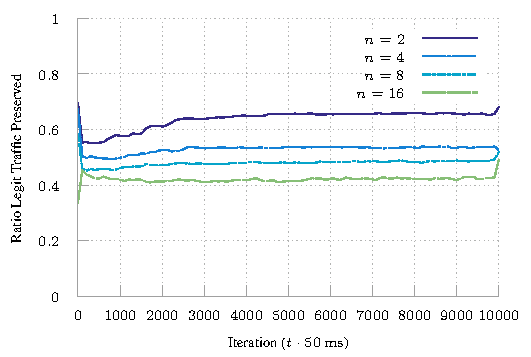
\includegraphics[width=0.90\linewidth]{../plots/online-varyN-binary}
	\caption{
		MARL pushback control system performance plotted over time for various settings of $n$ hosts per agent.
		This plot shows that, from the perspective of benign hosts, service guarantees degrade as inference and actions become less granular.
		This generalises for all behavioural discriminators: even a perfect agent \emph{must} punish benign flows if they are grouped with malicious actors.
		%		?? Effect on max perf AND learning rate??
		Crucially, both the maximum achievable performance and learning rate are negatively impacted when granularity is coarse.
		\label{fig:marl-granularity}
	}
\end{figure}

\Cref{fig:marl-granularity} shows that, as more hosts are allocated to each learner, the fraction of traffic believed to be good (as observed at the server) decreases.
This manifests in two ways: the best-achievable performance drops, and so too does the learning rate.
The first consequence arises analytically.
Given the probability that a host is legitimate, $P_G \in [0,1]$, it follows that a host will be malicious with probability $P_B = 1 - P_G$.
Defining \emph{imperfect service} to mean any case where all $n$ hosts connecting over a switch do not share the same classification (i.e., a mixture), then the probability that a switch is delivering imperfect service is $P_{M,n} = 1 - (P_G^n + P_B^n)$.
\begin{thm}
	As the host/learner ratio $n$ increases, it is more likely that a throttling switch will exhibit imperfect service: $\forall n \in \mathbb{Z}^{+}, P_{M,n} \le P_{M,n+1}$.
\end{thm}
\begin{proof}
	\emph{Base case:} $P_{M,1}=0, P_{M,2} = 1 - P_G^2 - P_B^2 > 0$.
	\emph{Inductive step:} Assume that the theorem holds for $n$. Observe that $P_G^n \ge P_G^{n+1}$ (resp.\ $P_B$). It then follows that:
	\begin{align*}
	P_G^n + P_B^n &\ge P_G^{n+1} + P_B^{n+1}\\
	1 - (P_G^n + P_B^n) &\le 1 - (P_G^{n+1} + P_B^{n+1})\\
	P_{M,n} &\le P_{M,n+1} \qedhere
	\end{align*}
\end{proof}
\begin{corr}
	Restricting $P_G \in (0,1)$ so that both $P_G$ and $P_B$ are non-zero ensures strict inequality: $P_{M,n} < P_{M,n+1}$.
\end{corr}

%?? Expand according to the summary you posted in the notes document.
%That the use of UDP-like traffic replicates their experiments, compared against how real tcp behaves in mininet and according to the Mathis equation, shows that they really did not consider the behaviour of benign TCP in this environ (i.e., their results should be considerably worse in practice).

\subsection{TCP Multiplexing and Falloff Behaviour}\label{sec:tcp-multiplexing-and-fallback-behaviour}

%While Tcpreplay was useful in recreating the original work and examining the above condition, flow behaviour under packet loss is closer to that of UDP when using it to replay traffic.
%To investigate the effects of collateral damage upon benign TCP flows, an iperf3 test was conducted using mininet.
%Several hosts communicated concurrently to a single server over one switch, with maximum send rates in $\{1,...,5\}$ \si{\mega\bit\per\second} and a constant \SI{40}{\milli\second} latency.
%The rate of packet drop was increased linearly from \SIrange{0}{40}{\percent} and the observed throughput for each host was measured, to show a trend and determine for the mininet environment whether throughput would decrease as expected, at a super-linear rate.

%\begin{figure}
%	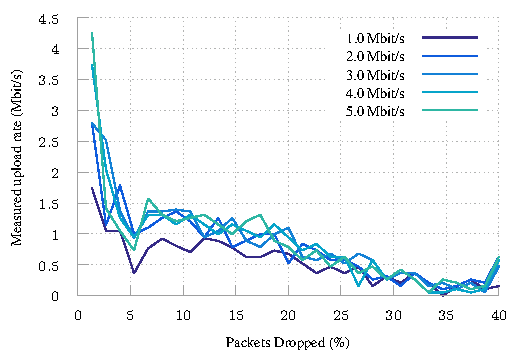
\includegraphics[width=\linewidth]{../plots/mplex}
%	\caption{
%		Average TCP upload rate of hosts targeting different bandwidths in \emph{mininet}, computed over 10 runs, for choices of packet drop rate up until throughput is reduced to almost \SI{0}{\mega\bit\per\second}.
%		As the rate of packet drop increases from \SIrange{0}{40}{\percent}, all flows converge on an extremely low throughput, regardless of the target bandwidth---a super-linear decrease for legitimate TCP traffic.
%		Prior treatments have ignored such phenomena, which have strong implications on agent and network design.
%		Malicious flows are not expected to obey the Mathis equation in this way, worsening collateral damage experienced by benign TCP flows.
%		\label{fig:mplex-tcp}
%	}
%\end{figure}

\begin{figure}
	\centering
	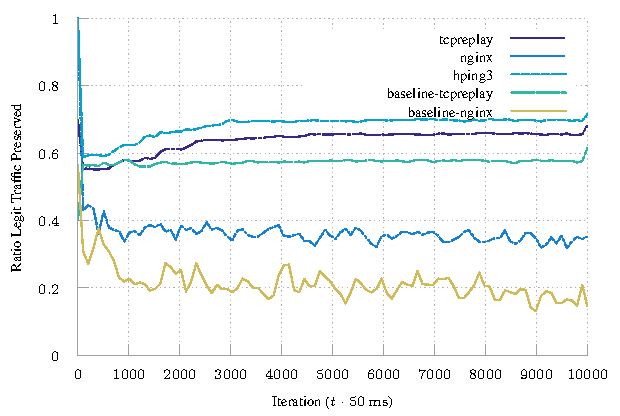
\includegraphics[width=0.95\linewidth]{../plots/online-varyN-nginx}
	\caption{
		Comparison of preserved traffic across different traffic models, choosing $n=2$ hosts per egress node.
		No actions are taken in the ``baseline'' entries.
		The agents examined here perform above the baseline in all cases, but perform significantly worse for live TCP traffic (nginx).
		\label{fig:nginx-coffin-nail}
	}
\end{figure}

%\Cref{fig:mplex-tcp} shows that this trend is present.
Given the UDP-like behaviour of Tcpreplay, replicating the online performance of \citeauthor{DBLP:journals/eaai/MalialisK15} in the $n=2$ case suggests that the numeric simulation their work is based upon does not capture the key interactions between TCP flows and packet drop as a control action.
To the best of our knowledge, existing RL applications for this task employ the same formulation with incremental improvements, and so such a deficiency would be likely to occur in \emph{all} these prior works.

From the Mathis equation \cite{DBLP:journals/ccr/MathisSMO97}, through which the performance characteristics of TCP under packet drop are well-known and well-understood, their results should be considerably worse in practice:
\begin{equation}
\operatorname{BW} = \frac{\operatorname{MSS}}{\operatorname{RTT}} \frac{C}{\sqrt{p}},
\end{equation}
for the \emph{maximum segment size} (MSS), \emph{round trip time} (RTT), a choice of constant $C \approx{} \sqrt{3/2}$ dependent on system assumptions, and the probability $p \in (0, 1]$ that a packet is lost.
?? TCP Cubic WAS used on the lab machines. We do still see Mathis-like behaviour with TCP Cubic, which is a significant observation.
?? Does Mathis still hold? We observed similar trends empirically, but perhaps not the \emph{exact} curve or falloff behaviour...
Accordingly, benign TCP flows are severely harmed by \emph{any} packet drop, so collateral damage to these hosts is more significant; good-faith TCP congestion avoidance causes these flows to attempt to back off very quickly.

TCP-Cubic still has a dependence on the $1/p^{0.75}$ -- slightly slower falloff, but still significant \cite{rfc8312}.

TCP traffic as it appears here is generated according to \Cref{sec:a-new-normal}.
\Cref{fig:nginx-coffin-nail} shows that this model performs poorly when attempting to safeguard TCP traffic, though it remains better than leaving the network unprotected.
%?? Talk about the same major points you made in the presentation here (i.e. TCP interactions) w/ pushback. Or in the evaluation...
UDP, however, behaves as expected---malicious hosts are expected to exhibit the same behaviour, given that congestion is their primary goal.

These results are of particular importance due to TCP's prevalence within the Internet.
The protocol is known to carry \SIrange{79}{94}{\percent} of packets, corresponding to \SIrange{89}{98}{\percent} of data transferred by volume \cite{DBLP:conf/saint/ZhangDJC09}.
?? NEED TO VERIFY VOLUME OF CONGESTION-AWARE TRAFFIC IN MODERN DAY WITH CAIDA.
As far as future network protocols are concerned, QUIC \cite{DBLP:conf/sigcomm/LangleyRWVKZYKS17}, a congestion-aware stream transmission protocol, will behave much like TCP, showing the importance of further development to properly handle traffic with such characteristics.

\subsection{Computational Cost}
%?? Consider talking about the execution times of the old MARL approach here? They're real nice (as expected), so we have lots of room to play around with while (hopefully) remaining under the 1ms target time given by \textcite{DBLP:conf/sigcomm/ChenL0L18}.

%Overall, each episode takes around \SI{10}{\minute} to run, while each set of \num{10} requires around \SI{2}{\hour} due to additional set-up/tear-down costs associated with mininet.
Measurements taken during each of these experiments indicated that the cost of computing any action is typically within \SIrange{80}{100}{\micro\second}.
This is reassuring when measured alongside the insights from other work.
\Textcite{DBLP:conf/sigcomm/ChenL0L18} observe that, ideally, actions must be computed and taken within \SI{1}{\milli\second} to have a meaningful affect on short flows.
%Most flows are short, and flow-size follows a heavy-tailed distribution.
That our starting point falls significantly below this threshold allows us to safely consider more costly actions or larger state spaces, which would typically increase the computational cost.

%\subsection{Synthesis}
%%It'd be really good if I could figure out a rough proof for the service property...
%%Okay... now say what this means for future viability! What changes can I make? Flow-specific metrics, of course! Increase granularity as much as I can!
%Both of these experiments suggest that the most viable way to enhance and deploy this MARL approach is to consider flows individually to maximise performance for legitimate hosts and to detect malicious hosts in a more principled manner.
%While this will add significant computational cost, this may be worked around with intelligent sampling and monitoring while taking multiple actions per-timestep \cite{DBLP:conf/hotnets/MaoAMK16}.
%
%?? Observations: training time lengthier by nature of emulated environment.
%?? Risk of going for a simulation (i.e. numeric)? Always going to be interesting behaviour that is missed out on (in theory), at the cost of training time/limits of simulation speed

\section{A New Normal}\label{sec:a-new-normal}

%In establishing...
%
%?? How will I structure this?
%?? Motivation -> Model -> Results?
%?? OR Use the results of the last section to springboard into here?

From what we have seen, it is difficult (or impossible) for trace-based or numerical simulations to correctly capture certain dynamics without an extraordinary amount of care or consideration.
%As it turns out, 
Our goal is to briefly describe an environment which tests \emph{specific} behaviours to examine the \emph{specific} problems which have arisen during our testing of past approaches.
We contribute a network model built around live testing of TCP traffic in an SDN-enabled environment, which is adaptable to arbitrary topologies, with an explicit focus on preserving the real-time dynamics of TCP traffic.
In particular, we are interested in capturing interactive, correlated back-and-forth exchanges associated with live HTTP traffic; mainly because of the particular interactions between the application-level dynamics, congestion awareness at the transport level and the nature of control signal used.
Naturally, this model is not perfect or representative for all traffic, yet it captures some of the behaviour which we expect will plague most legitimate TCP flows.
If need be, we expect the frequency or distribution of requests could be conditioned to match observations of real-world access patterns.

%?? ANGLE: set up an environment to test \emph{specific} behaviours to examine \emph{specific} problems in past work. I make no claims that it is perfect or representative for all traffic, just for this (likely common) behaviour which I expect to plague almost all legit TCP flows.

%?? Existing sims used for testing such applications reliant on traces, or not sophisticated enough to capture interactive, back-and-forth (correlated) behaviours---possibly discarded as second-hand effects by past work when these are so crucial given user traffic patterns (and the nature of the control signal we choose to enact).

%?? Remember, the motivation is clear. We don't care so much that it is "representative" wrt a specific deployment location or network type. The whole purpose of this is that we aim to test specific behaviour which traces cannot replicate (i.e., correlated back-and-forth, dynamics introduced to congestion-aware protocols, ...)
%?? If we need to, we can condition the distribution of requests according to statistics mined from an existing trace if reviewer number 2 needs that extra push to be convinced.

\subsection{Network Design}
We make use of a fully software-defined network, built using OpenFlow-aware switches in mininet alongside a controller application based on \emph{Ryu} \cite{ryu}.
All internal routers are primed with knowledge of the shortest path to each internal host, while new inbound flows register the ``way back'' for each hop used, to ensure consistent traffic conditions for each flow.
If such information is lost, perhaps expiring due to inactivity, it suffices to forward an outbound packet on a random (outbound) port, as we assume that any external IP is reachable through any of the test network's egress ports (i.e., that it is not connected to any stub autonomous systems).
The controller is also responsible for computing how switches respond to ARP requests: the necessity of this arises due to the reliance upon Linux's networking stack for live applications, and wouldn't need to be considered for purely trace-based evaluation.
We make further use of the topology presented earlier (\cref{sec:topology}), noting that our architecture allows us to trivially extend and modify this if required.

\subsection{Traffic Model}
%?? Legitimate traffic: TCP traffic (HTTP clients downloading web pages, dependent resources and files) with a mixture of lifetimes for each request.
To model legitimate traffic, the server node runs an nginx v1.10.3 HTTP daemon, serving statically generated web pages alongside various large files and binaries.
Benign hosts run a simple libcurl-based application written in Rust, repeatedly requesting resources from the server.
Each host's download rate is limited to match whatever maximum bandwidth was assigned to it.
This provides two modes of operation:
\begin{itemize}
	\item \emph{long flow} testing has each host constantly request a large binary file, such as a tarball of GCC8;
	\item \emph{request-chain} testing has each host request several random files known to exist within the website, followed by any dependent resources for each (stylesheets, images, etc.). On completion, a host changes its IP to generate separate statistics per-flow, while minimising downtime. This presents a more balanced distribution of flow duration and size.
\end{itemize}
We offer these to model two extremes: long-life host-to-server transfers (a characteristic we might expect from e.g., streaming video), and common HTTP traffic.

%?? Malicious traffic: UDP flood traffic (hping3, MTU-size packets, ). Why not min-size packets? Because the traffic generator gets in a horrible rut if I do so...
Malicious traffic is generated by use of the \emph{hping3} program, generating UDP-flood traffic targeting random ports.
Each malicious packet is MTU-sized, loosely mapping to the large frame sizes expected in an amplification attack and to ensure that emulation remains tractable.
When using TCP-like traffic, we must increase each attacker's upload range to \SIrange{4}{7}{\mega\bit\per\second} to meaningfully impact benign flows---a \SI{30}{\percent} rate increase in expectation, uploading \SIrange{2.03}{2.18}{$\! \times U_s$}.
The expected fraction of $U_s$ consumed by each host is \SI{21.5}{\percent} for $n=2$, and \SI{2.84}{\percent} for $n=16$.

\section{Acting On Individual Sources}\label{sec:acting-on-individual-sources}
Our main hypothesis is that the best method for advancing past the current shortcomings of RL-based DDoS mitigation is to modify the design of agents such that filtering decisions are computed per source.
However, any of these alterations must account for computational constraints imposed by the deployment environment---the amount of flows passing over an agent is unbounded.
We describe and justify our enhancements to the RL model of \textcite{DBLP:journals/eaai/MalialisK15}, present a new model which draws on domain knowledge leveraged by SPIFFY \cite{DBLP:conf/ndss/KangGS16}, and offer an empirical investigation into the effectiveness of flow-level statistics on live decision-making.

\subsection{Marl++}\label{sec:marl-plus}
%\fakepara{Multiple actions}
%?? Talk about the modifications to standard: multiple actions per-timestep, updating many traces from one reward...
Modifying the frequency with which actions and value functions are updated has important consequences for not only overall system performance, but also in \emph{how} an agent learns.
We choose to adapt these algorithms to prioritise rapid response to changes in network state and to visit as many state-to-state transitions as possible to facilitate effective learning.
To this end, we allow agents to make many decisions per timestep.
We maintain the last state-action pair associated with each source IP, and calculate any actions for the flows which still exist.
Finally, we update $\wvec{}$ according to \cref{eqn:sg-sarsa} with each available trace and the sole reward measurement an agent has at that time.
As exploration still occurs for each action, this approach reduces $\epsilon$ multiple notches every timestep.
In turn, we increase the annealing window for $\epsilon$ to \num{8000} action choices so as to preserve exploration over time, by accounting for the greater volume of decisions being made.

%\fakepara{Timed Random Sequential actions}
Taking actions in this manner means that any agents are assigned a larger, and potentially unbounded, set of tasks to perform every time they receive load and flow statistics from the network and their parent switch.
This introduces numerous potential issues: inability to respond to unexpected changes in flow state, delayed service of new flows, and risks that flow states become outdated; at their worst, these present additional attack surfaces to an adversary.
To adapt to these problems, we make use of \emph{timed random sequential} updates.
Each agent begins with an empty work list.
For the set of flows active in any timestep, we shuffle the list and perform as many action calculations and updates as possible, within a set time limit.
Uncompleted work is passed on to the next timestep, until the list is emptied, at which point is is repopulated using the set of available measurements.
To ensure that flow control actions are made with recent information, we combine state vectors for unvisited flows in the current work set, and replace the stored vector for all others.
State vector combination is done by summing deltas and packet counts, updating means via weighted sums, and replacing all other fields with the newest measurements.
Following \citeauthor{DBLP:conf/sigcomm/ChenL0L18}'s observations concerning short flows \cite{DBLP:conf/sigcomm/ChenL0L18}, we maintain a deadline of \SI{1}{\milli\second}---in tests, an agent is typically able to process around 8 flows in this time.
We expect this should be tuned based on the frequency at which statistics arrive.
%?? Prune old? We can get through 8 per iteration, might use this as a basis for knowing when to say ``enough is enough''.

\newcommand{\arrload}[2]{\operatorname{load}^{#2}_{t}(#1)}
\newcommand{\uload}[1]{\arrload{#1}{\uparrow}}
\newcommand{\dload}[1]{\arrload{#1}{\downarrow}}
\newcommand{\bload}[1]{\arrload{#1}{\updownarrow}}
\newcommand{\cond}[2]{\operatorname{c}_{#1,t}#2}
%\fakepara{Reward function directionality}
The reward functions, as defined, do not take traffic direction into account.
We redefine these to identify overload states using both upstream and downstream loads, while allowing customisation of which direction is chosen for protection.
Denoting the upstream, downstream and combined loads $\uload{s}, \dload{s}, \bload{s}$, we modify \cref{eqn:reward}:
\begin{subequations}
\begin{gather}
\cond{f} = [\max(\uload{s}, \dload{s}) > U_s],\\
\cond{c}{(v)} = \cond{f}{} \cdot{} \, [\max(\uload{l_v}, \dload{l_v}) > U_s/k],
\end{gather}
\label{eqn:reward-but-better}
\end{subequations}
replacing $\arrload{t}{}$ in \crefrange{eqn:reward-rt}{eqn:reward-rctl} with whichever directional load is prioritised.
We choose $\uload{\cdot}$ for our UDP-based models and $\dload{\cdot}$ for HTTP, though we expect that $\bload{\cdot}$ would be the most suitable for general deployment or heterogeneous traffic patterns.
These choices reflect where the bulk of transmitted bytes in each model are observed (and the lack of this knowledge in the general case).

%Explicitly mention \emph{why} we don't make use of neural networks, and instead favour more classical function approximation. Latency concerns, energy usage, graphics/TPU/whatever hardware availability or lack thereof across switches/routers/etc.
To make decisions cheaply and at low latency, we maintain the usage of semi-gradient Sarsa with tile coding, rather than making use of neural networks or more complicated function approximators.
Although this likely brings lower theoretical performance, there are more reasons than latency alone to favour classical methods; these include lower energy usage, reduced model complexity (and training time), the availability of necessary hardware, and simpler decision boundaries.
This aligns with our goal of quick online learning, and potentially faster adaptation to aggregate changes in traffic without necessarily introducing dedicated tensor processing hardware to networks.
Simpler decision boundaries reduce the risk of overfitting and of unexpected behaviour, and we anticipate that the simplicity of policy computation in the chosen manner will also greatly aid interpretability of anomalous action choices.

%?? Expand all this

\subsection{SPF: SPIFFY Lite}

An important question to ask while exploring the design space of RL agents is whether (and how) domain knowledge can improve the performance or learning rate of a defence system.
This often comes as a trade-off: expressive power and control, weighed against the smaller action spaces afforded by existing insight or structure.
We propose a second model, relying on the measurements of \textcite{DBLP:conf/ndss/KangGS16} which suggest that bot attack flows cannot scale up to match an increase in available bandwidth.
While it is not stated whether this behaviour applies to amplification attacks, we expect this to remain the case; the upload rate of any amplifier will be fixed at its upper bound given that the upstream links of any connected bots are saturated.
Moreover, bots receive no feedback on the effective throughput of their attack flows.

How might we apply their observations within the RL paradigm, while tailoring them towards non-ISP deployment?
Our approach is to constrain how an agent treats each flow using a simple finite state automaton: we restrict $p \in \left\{ 0.00, 0.05, 0.25, 0.50, 1.0 \right\}$, choosing to add complete filtering to a steady progression of rate-limiters (\SI{25}{\percent} increments for UDP traffic).
The outlier, $p=0.05$, corresponds to roughly a \SI{50}{\percent} rate reduction for TCP flows in our test topology.
This uneven spread of choices for $p$ allows light and heavy rate reduction to be applied to both congestion-aware and non-congestion-aware traffic as required.

The action set is then reduced such that agents can \emph{maintain}, \emph{increase}, or \emph{decrease} $p$ in single steps.
To enable temporary bandwidth expansion in resource constrained deployments, every flow is initially placed under light packet drop ($p=0.05$, or state 1); this is chosen above the equivalent for UDP due to TCP's higher prevalence.
We combine this with the enhancements described in \cref{sec:marl-plus}.

This model is significantly different when considering how to tune the RL algorithm's parameters: each agent now requires the capability to plan ahead, since they may no longer choose $p$ directly from any state.
This entails choosing some discount factor $\gamma \ne 0$, allowing the value of future states to influence state-action value updates.
Recounting \cref{sec:reinforcement-learning}, the choice of $\gamma$ affects which fraction of the current state-action pair's value is added to $R_t$ when updating the value of the last state-action pair.
We found the setting $\gamma = 0.8$ to be the most effective choice for this hyperparameter during exploratory testing with UDP traffic, by observing average performance over $\gamma$ increments of $0.1$.

\subsection{Rethinking the State Space}\label{sec:rethinking-the-state-space}

\begin{figure}
	\centering
%	\begin{subfigure}{0.32\linewidth}
%		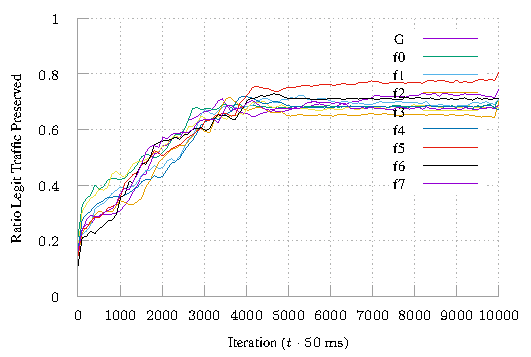
\includegraphics[width=\linewidth]{../plots/ftprep-good}
%	\end{subfigure}
%	\begin{subfigure}{0.32\linewidth}
%		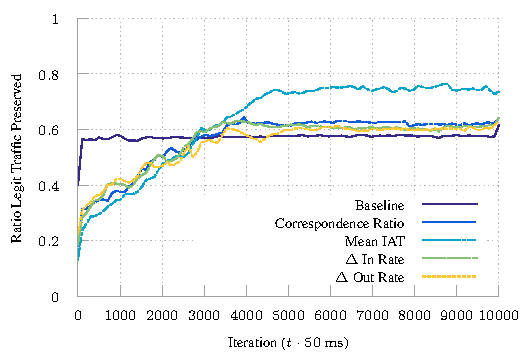
\includegraphics[width=\linewidth]{../plots/ftprep-good-2}
%	\end{subfigure}
%	\begin{subfigure}{0.32\linewidth}
%		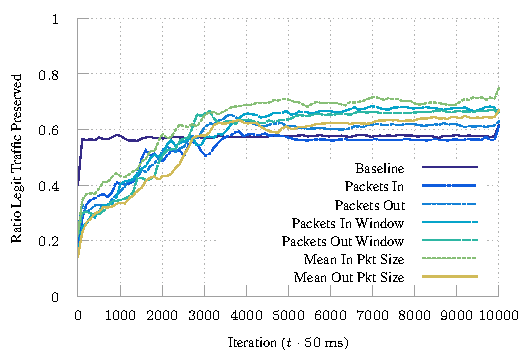
\includegraphics[width=\linewidth]{../plots/ftprep-good-3}
%	\end{subfigure}
	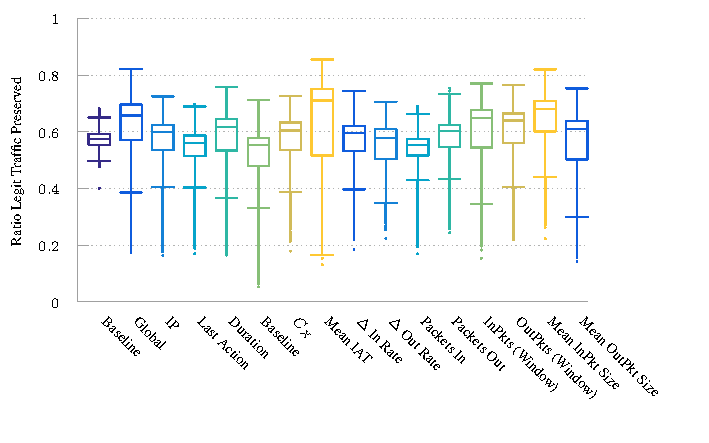
\includegraphics[width=\linewidth]{../plots/ftprep-box}
	\vspace{-1.2cm}
	\caption{
%		Features: how good are they really? These are for UDP. As you can see, Most things are pretty average (except for \emph{Mean IAT}, which dominates).
		Learned performance of Marl++ agents when benign traffic is UDP-like, using only a single feature as a basis for decisions.
		Mean IAT, inbound packet sizes, and global state offer the best predictive performance, while most features offer marginal advantage over the unprotected baseline.
		Here, the link's bandwidth limit is removed, and so agents automatically learn to keep bandwidth below $U_s$ by negative reinforcement---this offers a slight per-feature performance increase compared to when this explicit cap is present (not pictured).
		\label{fig:udp-feature-plots}
	}
\end{figure}

\begin{figure}
	\centering
	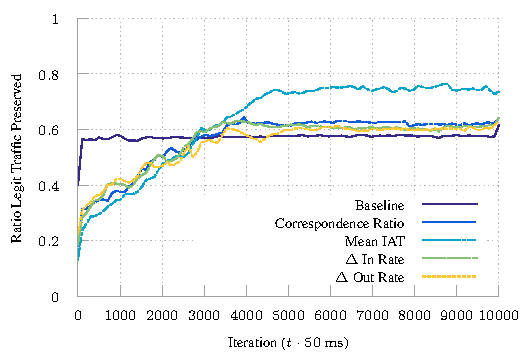
\includegraphics[width=0.9\linewidth]{../plots/ftprep-good-2}
	\caption{
		Demonstration of learning rate for several features included as part of \cref{fig:udp-feature-plots}.
		Performance starts low, before achieving convergence at some later time; this explains the high volume of outliers occurring below the main distribution of many features.
		\label{fig:udp-fp-converge}
	}
\end{figure}

%\begin{figure*}
%	\centering
%	\begin{subfigure}{0.32\linewidth}
%		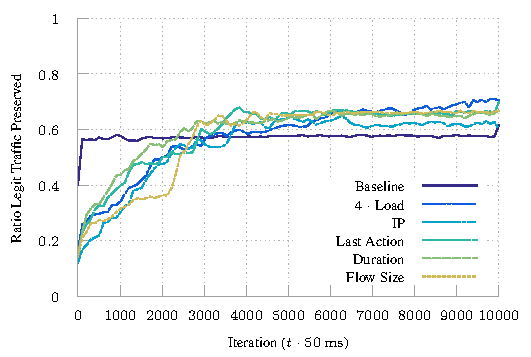
\includegraphics[width=\linewidth]{../plots/ftprep-cap-good}
%	\end{subfigure}
%	\begin{subfigure}{0.32\linewidth}
%		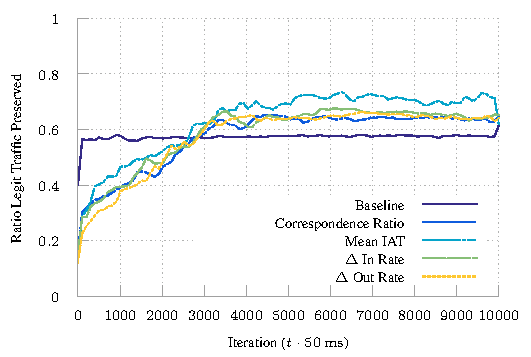
\includegraphics[width=\linewidth]{../plots/ftprep-cap-good-2}
%	\end{subfigure}
%	\begin{subfigure}{0.32\linewidth}
%		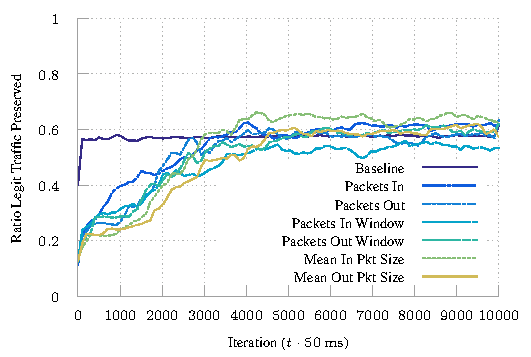
\includegraphics[width=\linewidth]{../plots/ftprep-cap-good-3}
%	\end{subfigure}
%	\caption{
%		Features: how good are they really? These are for UDP, but capped. As you can see, Most things are pretty average (except for \emph{Mean IAT}, which dominates).
%		\label{fig:udp-cap-feature-plots}
%	}
%\end{figure*}

\begin{figure}
	\centering
%	\begin{subfigure}{0.32\linewidth}
%		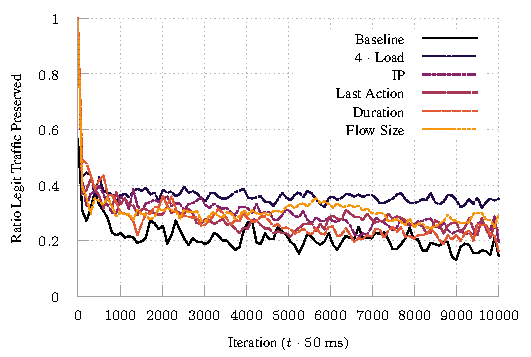
\includegraphics[width=\linewidth]{../plots/ftprep-tcp-good}
%	\end{subfigure}
%	\begin{subfigure}{0.32\linewidth}
%		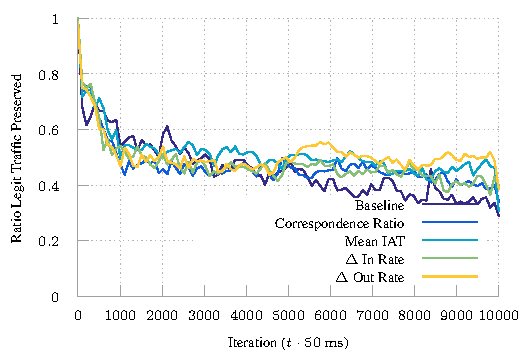
\includegraphics[width=\linewidth]{../plots/ftprep-tcp-good-2}
%	\end{subfigure}
%	\begin{subfigure}{0.32\linewidth}
%		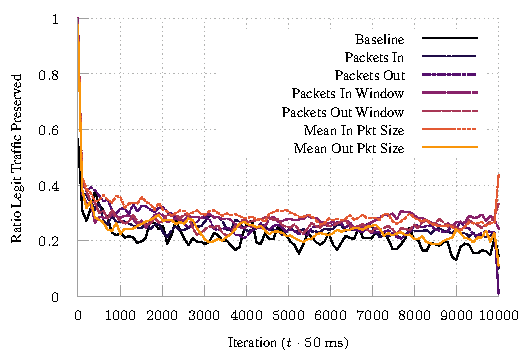
\includegraphics[width=\linewidth]{../plots/ftprep-tcp-good-3}
%	\end{subfigure}
	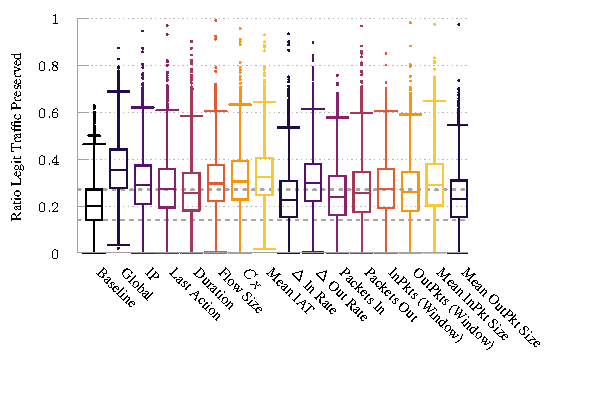
\includegraphics[width=\linewidth]{../plots/ftprep-tcp-box}
	\vspace{-1.2cm}
	\caption{
%		Features: how good are they really (part 2)? These are for TCP. These are less conclusive...
		Learned performance of Marl++ agents when benign traffic is TCP-like, using only a single feature as a basis for decisions (uncapped as in \cref{fig:udp-feature-plots}).
		Global state and Mean IAT still offer the greatest improvement above baseline, but it is observed that different optimal features are expressed between different traffic models.
		Packet-level statistics are considerably less effective for this class of traffic, with $\Delta$ Out Rate and Correspondence Ratio being proportionally better than they are for UDP.
		\label{fig:tcp-feature-plots}
	}
\end{figure}

\begin{figure}
	\centering
%	\begin{subfigure}{0.32\linewidth}
%		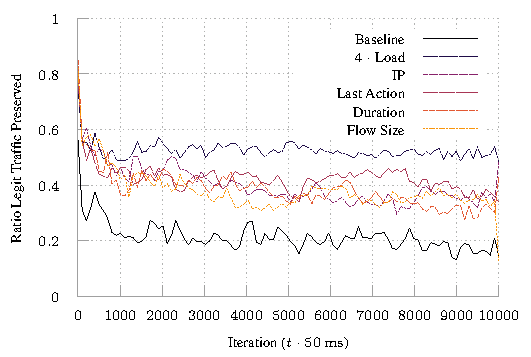
\includegraphics[width=\linewidth]{../plots/ftprep-tcp-cap-good}
%	\end{subfigure}
%	\begin{subfigure}{0.32\linewidth}
%		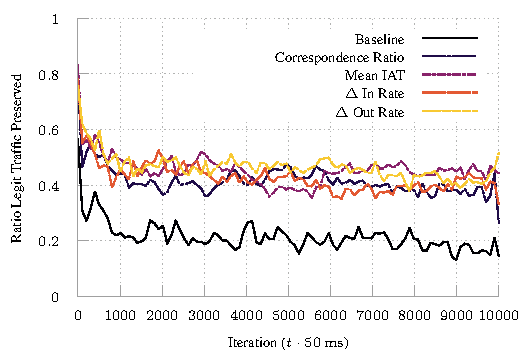
\includegraphics[width=\linewidth]{../plots/ftprep-tcp-cap-good-2}
%	\end{subfigure}
%	\begin{subfigure}{0.32\linewidth}
%		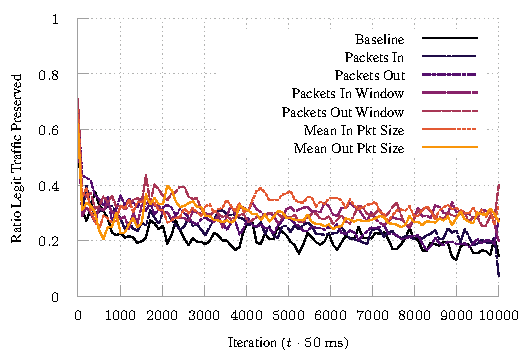
\includegraphics[width=\linewidth]{../plots/ftprep-tcp-cap-good-3}
%	\end{subfigure}
	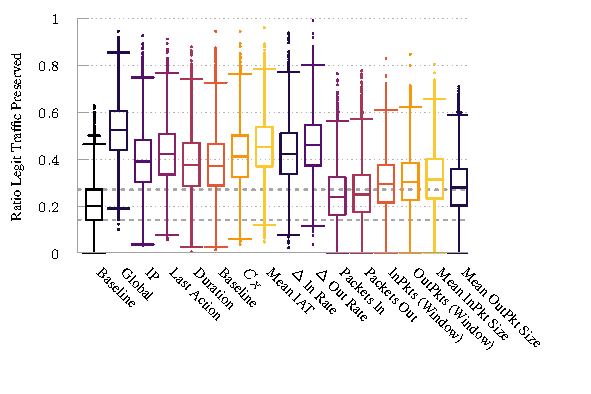
\includegraphics[width=\linewidth]{../plots/ftprep-tcp-cap-box}
	\vspace{-1.2cm}
	\caption{
%		Features: how good are they really (part 3)? These are for TCP, but capped. These are less conclusive...
		Learned performance of Marl++ agents when benign traffic is TCP-like, using only a single feature as a basis for decisions (with bandwidth capped physically).
		Although negative rewards (and thus negative reinforcement) cannot occur, all features achieve considerably better performance, a reversal of our observation for UDP traffic.
%		Global state and Mean IAT still offer the greatest improvement above baseline, but packet-level statistics are considerably less effective for this class of traffic.
		\label{fig:tcp-cap-feature-plots}
	}
\end{figure}

The main element required to move to a per-source model is a feature set which offers high predictive power, such that behavioural differences are readily apparent to an agent.
Elaborating further on the statistics discussed in \cref{sec:motivation} which others have shown to be effective, we believe the following features to be useful (and humanly justifiable), and offer an investigation into their use alongside different traffic types:
%?? We use these features, and why...

\fakepara{Global state}
These are the existing set of load measurements introduced in \cref{sec:environment-and-rl-algorithm}.
These indicate the overall health of the network, and crucially are all measurements which an agent directly controls.

\fakepara{Source IP address}
While ordinarily trivial to spoof (and thus of limited use for many classes of attack), reflectors are themselves legitimate services being abused by spoofing attackers.
As a result, they communicate with attack victims using their own IP address.
In real-world scenarios the addresses of a set of reflector nodes might exhibit similarity, e.g., similarly unhardened services exposed by a single organisation.
?? Can we support this claim?

\fakepara{Last action taken}
This encodes an agent's current belief in the maliciousness of a flow.
This feature also potentially allows forgiveness, serving as a reference point for determining whether a source mistakenly marked as malicious exhibits different falloff behaviour after punishment.

\fakepara{Flow duration and size}
Features which describe the length of time a connection has been active, and the amount of data transferred within that time.
An extraordinarily long flow, having sent a lot of data, could be more likely to be an amplifier: though most (\SI{62}{\percent}) waves of amplifier traffic last shorter than \SI{15}{\minute} \cite{DBLP:conf/raid/KramerKMNKYR15}, this is considerably longer than the typical length of an HTTP request/response.

\fakepara{Correspondence ratio}
The ratio between upstream and downstream traffic for a source IP.
We define this to be $C_X = \min(\uload{\cdot}, \dload{\cdot})/\max(\uload{\cdot}, \dload{\cdot})$, where a value close to 0 indicates strong asymmetry.

\fakepara{$\mathbf{\Delta}$ Send/receive rate}
The change in traffic rates caused by the last action.
Behavioural changes induced by bandwidth expansion/reduction are expected to be most visible in these fields.

\fakepara{Mean inter-arrival time (IAT)}
A measure of how often packets arrive at the agent's parent switch; low IATs indicate a high number of packets per second, and can be a possible marker of malicious behaviour.
We only make use of the mean IAT of \emph{inbound} traffic.

\fakepara{(Per-window) packet count}
The amount of packets sent to/from a source over a flow's lifetime (or the current window of measurement), similar in use to flow size and mean IAT.

\fakepara{Mean packet size per window}
Legitimate flows, both TCP- and UDP-based, often transmit packets with a distribution of sizes.
Attack traffic is not likely to be so diverse: we might expect solely max-size packets in the case of amplification attacks, or minimum-size packets in other classes of flooding attack.

The exclusion of features such as source/destination ports or protocol numbers is a deliberate choice.
If \emph{QUIC} (or a similar protocol) were to become ubiquitous, then these fields would have little to no correlation with the class of traffic a flow might contain.
Our aim was to design around this constraint as a form of future-proofing.

\begin{table}
	\centering
	\caption{Tile coding windows for each feature.\label{tab:codings}}
	
	\begin{tabular}{@{}ll@{}}
		\toprule
		New Feature (unit) & Range \\
		\midrule
		Load (\si{\mega\bit\per\second}) & $[0, U_s]$ \\
		IP & $[0, 2^{32}-1]$ \\
		Last Action (\si{\percent}) & $[0, 1]$ \\
		Duration (\si{\milli\second}) & $[0, \num{2000}]$ \\
		Size (\si{\mebi\byte}) & $[0,10]$ \\
		Correspondence Ratio & $[0,1]$ \\
		Mean IAT (\si{\milli\second}) & $[0, \num{10000}]$ \\
		$\Delta$In/Out Rate (\si{\mega\bit\per\second}) & $[-50, 50]$ \\
		Packets In/Out & $[0, 7000]$ \\
		Packets In/Out Window & $[0, 2000]$ \\
		Mean In/Out Packet Size (\si{\byte}) & $[0, 1560]$ \\
		\bottomrule
	\end{tabular}
\end{table}

All of the above features, save for global state, are 1-dimensional.
Each is tile-coded with 8 tilings and 6 tiles per dimension, using the windows described in \cref{tab:codings}.
We chose to take a separate tile-coding over each feature, ignoring combinatorial effects at present to minimise the amount of extra work an agent must perform.
Indeed, combining too many features into one tile-coding can lead to poor performance due to an inability to generalise action values across similar states.
On the other hand, treating features individually allows us to reach a quick understanding of the importance of each while seeing adequate performance.

\Cref{fig:udp-feature-plots} shows the effectiveness of each feature for UDP (resp.\ \cref{fig:tcp-feature-plots} for TCP), using a topology with $n=2$ hosts per egress point averaged over 10 episodes.
%?? Core findings---different protocols need different features, so everything we proposed above has a use!
The plots demonstrate that different protocols and traffic classes are best defended by different features---as such, every feature presented has value in a complete model.
All features converge to their highest-observed performance within around \num{4000} timesteps: \cref{fig:udp-fp-converge} shows an example of this behaviour for differently performing features.
In general, some of the most effective features are the global state, mean IAT, mean inbound packet size and $\Delta$ rates.
%?? How do they do when combined after individual training? Pretty well, especially for TCP.
Additional testing shows that the learned per-feature policies may be easily combined (by summing action values), and that this technique is particularly effective for TCP; these results are omitted to preserve space.
In no cases, however, do we manage to completely block attack traffic---at convergence, we observe that system load remains consistently at $U_s$.

?? POTENTIALLY CUT THE ``SYSTEM DYNAMICS'' AND/OR BANDED REWARDS, THEY DON'T ADD MUCH ANYWAY.

%?? NEED TO SAY SOMEWHERE: Baselines use TC for establishing interleaving/buffers filling etc., when MARL+ or SPF are in play then disabling TC (thus allowing illegal states, with \num{-1} reward marking them as such---``negative reinforcement'') may accelerate learning. We have a choice---but the results show that for TCP we WANT TC enabled... For UDP, we actually get a slight degradation in performance. This suggests a kind of ``banding'', perhaps? Important to mention that it easily learns how to maintain a logical bandwidth limit.
During training of the above feature models, we elected to remove the physical bandwidth limit to allow agents to visit illegal states and receive \emph{negative reinforcement} for doing so.
While this means that agents must learn how to keep traffic below a logical limit, they are helped by the fact that strong negative reward signals offer explicit information about which actions are poor choices: observe from \cref{eqn:reward,eqn:reward-but-better} that if a physical link has limit $U_s$ then we will never see a reward below 0.
It is important to note that neither setting affects the agents' ability to keep the total load below $U_s$.
%?? talk about cap difference: \cref{fig:tcp-cap-feature-plots}---we want cap enabled for TCP.
We found this led to a marginal improvement in efficacy when UDP was the primary source of benign traffic, but observed that this hindered learning when TCP was the primary protocol under protection (\cref{fig:tcp-cap-feature-plots}), likely due to the loss of key system dynamics.
It is anticipated that this difference might prove problematic for heterogeneous traffic mixtures.
One way of solving this may be to investigate the effect of replacing $U_s$ with e.g., $0.99 U_s$ in \cref{eqn:reward-but-better}, to introduce a small band of negative reinforcement without actually removing the load restriction in the environment.
It is crucial to make this region as small as possible, hence the somewhat arbitrary choice of factor; we observe that agents are always able to learn how to keep traffic consistently below the logical bandwidth limit (as in the original work).
Our intent is to potentially accelerate learning while preserving the effects of system dynamics---we term these \emph{banded} rewards.

%\subsection{What's done with these?}

%?? Tile coded together, action taken per-flow every timestep.

%?? NOTE: think about how I might need to change/alter the tile-coding when we add extra discriminative features... (i.e., are there better ways to handle covariance between properties of system/flow state, properly capture generalisation?)

%?? What other consequences are there? We're training each agent on all the flows it's acting on which means slight theoretical changes (we have multiple experience traces, and each uses its last state + new state + new target value (reward) as an update to the \emph{current model}).

\section{Results}
\label{sec:the-results-of-doing-so}

We now examine the performance of our two new models (\emph{Marl++}, \emph{SPF}) as compared against existing RL work (\emph{Marl}) under different traffic behaviour and varying $n$ as before.
%?? Probably best just to look at top level stuff, and THEN a simplified comparison for each intended improvement (like banded rewards).
Additionally, we examine the performance effects of environmental characteristics and potential improvements: negative reinforcement, the case where one agent makes all decisions, and pre-training on individual features.

We present the average rewards for all combinations of these factors in \cref{tab:av-vals}---these provide a rough idea of expected performance, giving the highest-performing model in bold.
Average rewards take into account any portions of time that an agent allows illegal system states.
Several plots augment this, illustrating peak performance or the amount of time which an agent requires to learn.

Unless stated otherwise, these experiments measure average performance over 10 episodes, use all \num{14} features introduced in \cref{sec:rethinking-the-state-space} (tile-coded individually) alongside the global state, and make use of the physical bandwidth cap rather than pursuing negative reinforcement.
In all cases, agents learn control of the network from scratch ($\wvec{}=\bm{0}$).
Test system specifications match those given in \cref{sec:performance-in-an-emulated-environment}.

\begin{table*}
	\centering
	\caption{Average reward for combinations of model, host density and traffic class.\label{tab:av-vals}}
	
	\expandableinput ../tables/big-avg-reward.tex
\end{table*}

\subsection{Congestion-unaware traffic}
%\begin{figure}
%	\centering
%	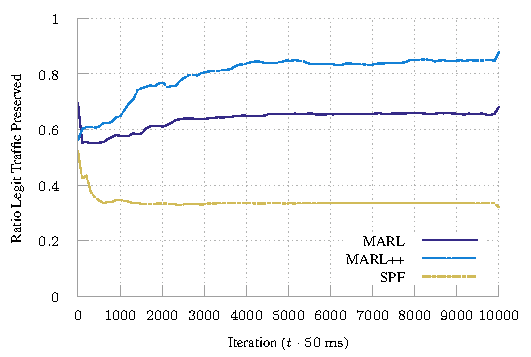
\includegraphics[width=0.9\linewidth]{../plots/udp-2}
%	
%	\caption{
%		Online performance for $n=2$ hosts per egress point when benign traffic is UDP-like.
%		Although Marl++ offers a marked improvement (a peak $\sim$\SI{30}{\percent} more benign traffic arrives unimpeded), SPF significantly underperforms for this relatively simple topology.
%		Non-SPF agents start off reasonably well, slowly learning better policies.
%		\label{fig:udp-2}
%	}
%\end{figure}
%\begin{figure}
%	\centering
%	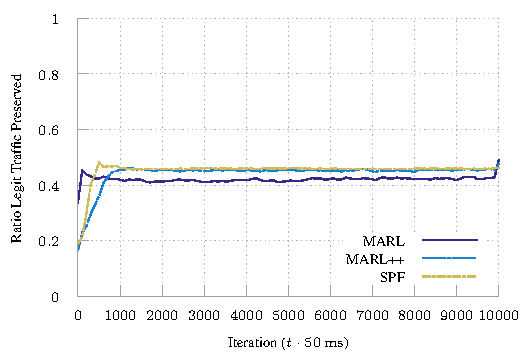
\includegraphics[width=0.9\linewidth]{../plots/udp-16}
%	
%	\caption{
%		Online performance for $n=16$ hosts per egress point when benign traffic is UDP-like.
%		Marl++ remains marginally ahead of its predecessor, though both have undergone a significant drop in effectiveness.
%		SPF, remarkably, displays performance on par with Marl++ for this more difficult topology.
%		Both of the new models take longer to train, but achieve better peak and average performance than Marl.
%		\label{fig:udp-16}
%	}
%\end{figure}
\begin{figure}
	\centering
	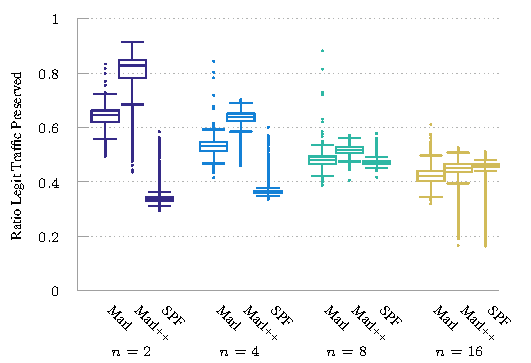
\includegraphics[width=0.95\linewidth]{../plots/udp-box}
	
	\caption{
		Online performance for UDP-like benign traffic.
		Marl++ offers a marked improvement (a peak $\sim$\SI{30}{\percent} more benign traffic arrives unimpeded) at small $n$, and remains marginally ahead of its predecessor by $n=16$, though both have undergone a significant drop in effectiveness.
		SPF, remarkably, slightly outperforms Marl++ (with lower variance) for this more difficult topology despite being worse for smaller $n$.
		Both of the new models take longer to train, but achieve better peak and average performance than Marl.
		The longer tails of outliers typically indicate the longer training time the new models require---we observe that SPF typically has considerably lower variance once it has converged on a stable policy.
		\label{fig:udp-box}
	}
\end{figure}

Across all choices of $n$, we see that Marl++ exhibits reduced collateral damage compared to Marl, with SPF starting poorly yet becoming more effective for larger $n$ (\cref{tab:av-vals}, \emph{Capped}, UDP).
\Cref{fig:udp-box} shows the behaviour for all choices of $n$---specifically, we see that Marl++ typically remains ahead of Marl, though this performance difference shrinks as $n$ increases, while SPF performs better at high host-density.

\subsection{Congestion-aware traffic}
%\begin{figure}
%	\centering
%	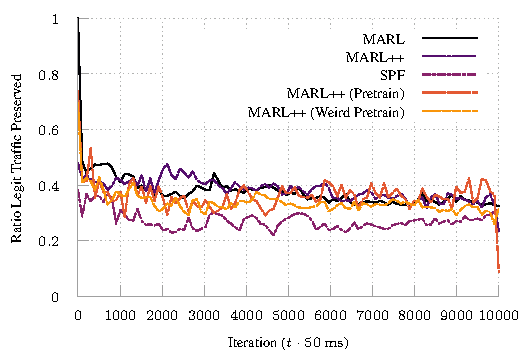
\includegraphics[width=0.9\linewidth]{../plots/tcp-2}
%	
%	\caption{
%		Online performance for $n=2$ hosts per egress point when benign traffic is TCP-like.
%		Marl++ and Marl achieve very similar performance, starting off similarly well without notable improvement over an episode.
%		SPF's performance is disappointingly close to baseline, indicating that it is as useful as having no defence system.
%		\label{fig:tcp-2}
%	}
%\end{figure}
\begin{figure}
	\centering
	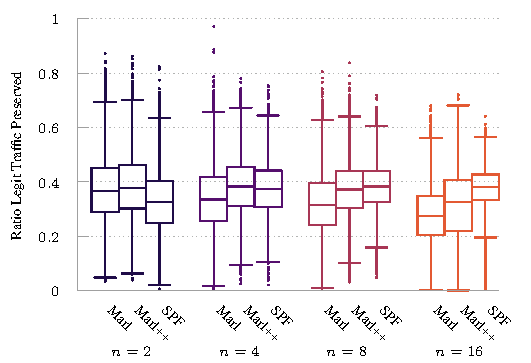
\includegraphics[width=0.95\linewidth]{../plots/tcp-box}
	
	\caption{
		Online performance for TCP-like benign traffic.
		Marl and Marl++ begin with essentially identical efficacy, with Marl++ having a small advantage at larger $n$.
		SPF is slightly worse than Marl and Marl++ at low $n$, but achieves considerably better median performance and lower variance than the other models for large $n$.
		\label{fig:tcp-box}
	}
\end{figure}
\begin{figure}
	\centering
	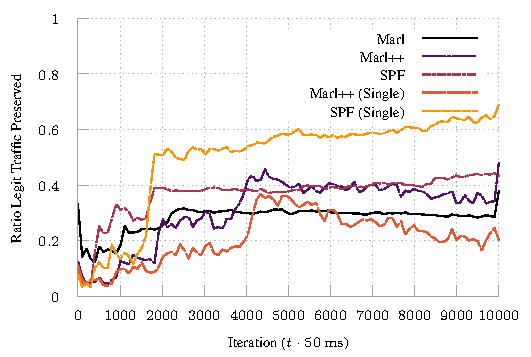
\includegraphics[width=0.95\linewidth]{../plots/tcp-16-single}
	
	\caption{
		Online performance of standard and single-agent models with $n=16$ hosts per egress point and TCP-like benign traffic.
		At this level of host density, SPF reaches its peak performance sooner and is considerably more consistent throughout the episode.
		Marl++ takes longer to reach its most effective policy, and achieves visibly better peak performance than the other standard models.
		With a single agent, Marl++ shows worse performance, while SPF improves significantly and continues to learn well past annealing $\epsilon \rightarrow 0$.
		\label{fig:tcp-16}
	}
\end{figure}

From \cref{fig:tcp-box}, Marl++ consistently allows more legitimate traffic to reach its destination than Marl, with both significantly above the baseline (\cref{tab:av-vals}, \emph{Capped}, TCP).
SPF performs slightly worse at low $n$, but outperforms both models as host density increases.
\Cref{fig:tcp-16} shows a trend in our results: for larger $n$, Marl++ requires around twice as long as Marl to learn its best-achieving policy, under-performing for this period, but achieves notably better peak and average performance.
SPF reaches a stronger plateau before \emph{both}, remaining more consistent and appearing to continue learning.

\subsection{Banded rewards and negative reinforcement}
?? PROBABLY CUT THIS

In general, we find that explicitly training a policy to keep the system in a valid state via negative reinforcement (i.e., an \emph{uncapped} network) is most effective for UDP-like traffic with Marl++.
For SPF, however, negative reinforcement is typically a worse choice.
Where TCP-like traffic is concerned in both models, we see that this strategy almost always leads to worse policies and higher collateral damage.

The usefulness of banded rewards with regard to learning an effective policy appears to be unpredictable.
For many of the configurations detailed in \cref{tab:av-vals}, for $n>2$ the average reward with banding is likely to lie between that of the capped and uncapped system models, but oscillates heavily.
In a handful of UDP instances, banding can lead to \emph{better} average performance.
More study is likely required into this; we replace $U_s$ with $0.99U_s$ to minimise the impact on legitimate states, but this choice remains somewhat arbitrary.

\subsection{Single-agent performance}
Making all decisions with a single agent is roughly equivalent to having a zero-cost communication channel between each pair of agents, theoretically allowing faster training by giving each agent more experience.
Curiously, we observe that this often leads to drastically worse policies when used as part of Marl++ for small $n$, but makes SPF a considerably more competitive model---especially for TCP, and as $n$ grows larger (\cref{fig:tcp-16}).
Single-agent SPF almost consistently outperforms Marl.
We discuss our conjectures for why this reversal occurs in \cref{sec:discussion}.

\subsection{Per-feature pre-training}
To investigate the effects of pre-training individual features, we chose our four best-performing features (global state, mean IAT, $\Delta$ in/out rates) and trained each over \num{10000} iterations, before evaluating the policy obtained by summing the action values suggested by each.
This may be achieved in a real network by randomly assigning new hosts to be controlled exclusively by one feature's policy, allowing agents to more easily learn \emph{which} information led to the correct action being taken.
To reflect this (and train all parts of an agent in the same time frame), we reduce the timestep length to \SI{10}{\milli\second} to train each agent in less wall-clock time, at the cost of noisier data (and reduced learning rate).
The results show little change for Marl++, but generally indicate a considerable gain for SPF (though smaller than what we'd measured for a single agent system).
%It's most likely that SPF is sensitive to noisy data when trying to learn how to act on TCP, and that as the different protocols did in \cref{fig:udp-feature-plots,fig:tcp-cap-feature-plots}, Marl++ and SPF have different optimal feature sets for different traffic behaviours---many of which may have been excluded.

\section{Discussion}\label{sec:discussion}

%Talk about flaws here, what could go wrong...

%?? Why does SPF only do well sometimes? Model is actually more difficult to learn, so it seems to do best when it has a larger set of decisions to learn from. But, it does worse for TCP?
\fakepara{Model performance}
Of the results presented, SPF's unpredictable (often worse) starting performance is unexpected, given its far smaller action space.
It's natural to expect that this would make the model easier to learn, but the additional state required appears to make the task \emph{harder}, beyond even the value of choosing a non-zero discount factor (adding forward-planning to explicitly mitigate this effect).
Accordingly, we see that SPF performs best when agents learn from as much knowledge as possible: high $n$ and single-agent training.
Why does it exhibit considerably lower variance?
Our belief is that SPF is, in fact, a considerably stronger model for these reasons, and its successes give us particular cause to consider the best schemes for efficient information sharing.
To filter incoming traffic from a source, it must decide to degrade their inbound traffic multiple times in a row, reducing the likelihood that a legitimate flow is punished by accident.
Paradoxically, Marl++ generally achieves the best performance yet actively suffers when trained as a single learner---this may occur due to a roughly even spread of values between disparate actions, due to shared characteristics between legitimate and malicious flows.

%?? May be hard to learn multiple features at once while controlling multiple flows while contending with many more agents, with harder dynamics like TCP. Does this hinder learning in the long run?
Although we have improved upon Marl in both identified problem cases, the improvements are not quite on the order we'd expect, or hope for.
%?? I don’t know if you want to also mention the problem of things getting “stuck” in locally optimal (but globally sub-optimal) policies. I think it’s fairly uncontroversial that an increase in state space would make this more likely. Also, the lack of discounting could play a large role (and more so as the state space becomes more complex…
The most likely explanation is that agents are converging to, and becoming stuck in, locally optimal (but globally sub-optimal) policies.
The increased state-space size makes this a more likely occurrence, as is the unclear affect of hyperparameters ($\alpha$, $\gamma$) as we scale up the state-space.
We suspect that these difficulties may be exacerbated by the competitive nature of learning that these models embody: agents are learning action values for multiple features simultaneously, taking many actions at once (making it harder to observe the true value of each action), and controlling shared global state.
Our pre-training results support the idea that it may be worthwhile to extensively pre-train agents non-competitively on each feature using individual flows.

%It is likely that the design of Marl++ 

%Finally, it is crucial to note that the models and techniques presented here are an improvement , this work still trails behind existing (exact) DDoS flow detection mechanisms.
Most importantly, what we wish to impart is the knowledge that while the models and techniques we present here are a significant improvement over past RL-based work, this work still trails behind existing (exact) DDoS flow detection mechanisms.
Although we have conducted work to map the territory to some extent, there are still more advancements to be made before RL-based DDoS defence is truly competitive.
The benefits we have at present are, however, substantial.
What we offer above the alternate approaches we discuss in \cref{sec:related-work} are potentially more flexible deployments and low-overhead decision-making, without requiring active measurement or the network resources and capabilities that the most effective techniques rely upon.
Moreover, our decision making processes are entirely agnostic of the protocol or content of inbound traffic, offering future-proofing against the introduction of new transports.

\fakepara{Security concerns and vulnerability}
Can an agent be flooded with new flows to reduce their ability to make decisions?
One of the risks introduced by our timed random sequential policy updates is that so much work can be queued up that an agent is never able to act on some attack flows.
The natural solution is to impose an upper bound on the amount of action computations/policy updates that can be performed before a work list is discarded completely.
This removes the guarantee that all flows will be visited fairly often, but if updates occur regularly then this random sampling may be sufficient to achieve good performance.

\begin{figure}
	\centering
	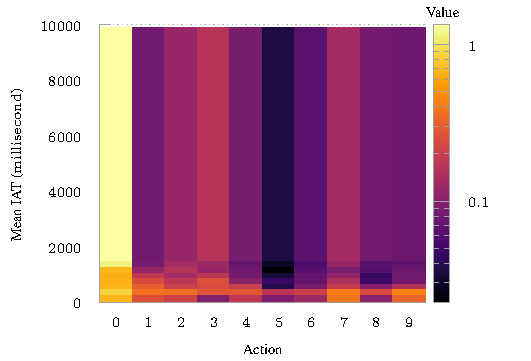
\includegraphics[width=0.9\linewidth]{../plots/policy-16-tcp-f5-mean-log}
	
	\caption{
		Mean Marl action values from pre-training on mean IATs ($n=16$).
		As these are mean values, lighter cells in each row indicate actions \emph{likely} to be taken by an agent's policy.
		Repeated values originate from the bias tile, which is always active, and indicate regions of the state-space which have yet to be visited---here, this is most of the state space.
		Agents visibly learn action values for tiles which override the default bias tile's preferences.
		The measured effectiveness of this feature then suggests that a low-resolution coding over the standard region may, in fact, be a better choice.
		We see that agents prefer to choose $p=0.0$ in most states, but higher $p$ when IATs are particularly small.
		\label{fig:intern-16-tcp-iat}
	}
\end{figure}

\begin{figure}
	\centering
	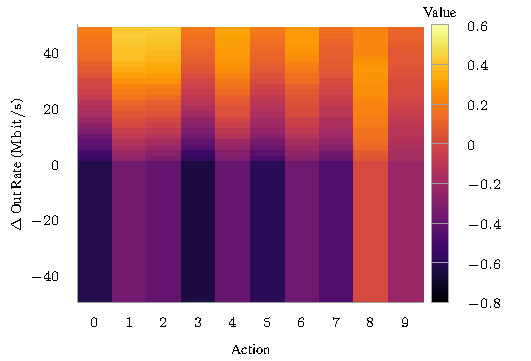
\includegraphics[width=0.9\linewidth]{../plots/policy-4-tcp-f7-mean}
	
	\caption{
		Mean Marl action values from pre-training on $\Delta$ out rates ($n=4$).
		A sudden ramp-up of server-to-host traffic is used as a strong indicator of flow legitimacy, while more punishing actions have comparatively higher value as $\Delta$ out rate decreases.
		Furthermore, we see again that a region of the state space has gone somewhat unexplored---we observed after plotting this visualisation that many decreases in this feature are too small to hit the adjacent tile, which implies a mixed-resolution coding may improve an agent's policy further.
		\label{fig:intern-16-tcp-something}
	}
\end{figure}

%?? Is the state space interpretable? Yes!
Machine learning algorithms have earned a reputation for eluding human interpretation, while being vulnerable to evasion and poisoning.
Given the risks associated with introducing such techniques in the context of security, it is natural to be concerned with the interpretability of the models we have proposed.
With the exception of global state, the tile-coding parameters we make use of ensure that the set of all outputs for each new feature we add is relatively enumerable: for $n$ tilings and $c$ tiles per dimension there are $nc^{\dim{f}}$ individual action value vectors per feature $f$ (\num{48} for the new features we introduce, \num{10368} for global state), though considerably more combinations thereof ($c^{n \cdot \dim{f}}$).
\Cref{fig:intern-16-tcp-iat,fig:intern-16-tcp-something} show how we may visualise the portion of a policy for each feature, and describe what information can be gained from doing so.
Furthermore, system state which is dependent on many signals drawn from across a wide network (such as our global state) is difficult to exert precise control over.
These signals' topological separation, in concert with their burstiness and unpredictability, may have substantial effects on an attacker's capabilities.

\fakepara{Real-world Deployment}
Currently, we assume that switches support an extension to OpenFlow to enable remotely installable packet-drop rules, either by running a modified version of OVS on commodity hardware at these locations or through custom firmware for egress switches.
Similar functionality could be employed by making use of OpenFlow's meter rules.

Where overheads are concerned, the state space sizes guarantee that a Marl policy remains under \SI{427}{\kibi\byte}, although in practice our sparse representation typically leads to far smaller policies: \SIrange{16.5}{17.0}{\kibi\byte} from our experiments.
As we have described earlier, action updates require a constant number of floating point operations---\num{122} floating point additions and \num{2} multiplications per update of $\wvec{}$, above the \num{140} additions required to choose an action.
The vast majority of these operations can be vectorised trivially, if such hardware is present.
Action computation for SPF is cheaper still, requiring only \num{42} additions per action required.
Beyond this, we require that egress switches are capable of co-hosting an agent (i.e., through \emph{network function virtualisation}), with the necessary hardware to support this choice.
We believe that it may be possible to implement similar behaviour on standard commodity switches through application of \emph{programmable data planes} \cite{DBLP:conf/ancs/JouetP17}.

%?? Incorrect, pickling...
%?? deployment/system guidelines, architecture, and overhead/footprint of doing this
%?? Mention: probably fewer state measurements than in our emulations, but longer measurements means less noisy (so probably more accurate)
Gathering and transmission of load/flow statistics would be difficult to perform quite as often as an emulated environment allows, without inadvertently affecting host traffic.
However, the measurements acquired in such a scenario are far more likely to be less noisy (by being collected over longer periods of time), which could aid effective training.
The main bottlenecks are most likely in forwarding the load measurements from various aggregation points (which can be made more efficient through multicast) and in running some estimator to condition the reward function upon.
%?? Potential for dividing up pre-feature training across different agents, or train like this locally (sets of flows trained by 1 sub-model).
%?? Different global state per-agent? Seems this must be locally trained, just make it (everything up the chain to key destinations).
We expect that agents will be able to share policies for all features, which may help to offset the reduced rate of incoming experience.
Regardless, it will take longer to achieve enough state-state transitions to converge on a good policy.

\section{Related Work}\label{sec:related-work}

%?? Try and compare my work here when possible?

\fakepara{DDoS Prevention}
\Textcite{DBLP:conf/lcn/BragaMP10} have examined the detection of ongoing (flooding-based) DDoS attacks through \emph{self-organising maps}, making use of SDN to gather statistics effectively.
Many of their features aren't overly relevant, as their focus is not active defence or discovering \emph{which} hosts are contributing to an attack.

?? Actually talk about Marl (???) to appease reviewer \#1.

\emph{SPIFFY} \cite{DBLP:conf/ndss/KangGS16} aims to remedy transit-link attacks by observing how flows from each source respond to a sudden increase in available bandwidth.
\Citeauthor{DBLP:conf/ndss/KangGS16} realise that bots participating in an attack are often unable to match this bandwidth expansion due to having already saturated the capacity of their outbound links, while legitimate flows typically speed up to match the new fair-share rate.
%Attackers must either be detected or reduce the throughput of each bot, increasing the cost of launching an attack.
Unlike our approach (and due to the class of attacks it is designed to defend against), SPIFFY is intended to be deployed within ISP networks, although some of our feature choices are backed by similar observations.
?? Flaws? what can't it do that we can do better? Long times to compute TBE routes on real networks, low expansion factor in real network can require more ``rounds'' of filtering. (``takes only'' \SI{14}{\second} for Cogent network? gross.)

\emph{Athena} \cite{DBLP:conf/dsn/LeeKSPY17} is a more generalised SDN framework for intrusion detection, but has shown the use of a \emph{k-nearest neighbours} classifier to detect individual attack flows.
Although heavyweight (and proven to be effective compared with \textcite{DBLP:conf/lcn/BragaMP10}), their comparison against SPIFFY lacks the quantitative evidence required to understand how the system compares.

\Textcite{DBLP:conf/sp/SmithS18} present techniques based on AS-level routing to tackle both transit-link and flooding-based attacks.
This view is taken due to the perceived cost of per-stream classification and inherent sensitivity to adversarial examples or crafted input.
The approach is creative, relying upon BGP \emph{fraudulent route reverse poisoning} to preserve traffic to a target AS, but unlike SPIFFY the approach doesn't actually \emph{remove} the congestion.
Because of this, traditional flooding-based attacks aren't fully alleviated.

%?? Abuses of RL 
\fakepara{RL in Networks}
Earnest, well-considered application of RL towards the challenge of intrusion detection/prevention has seen comparatively little examination.
Past work exhibits treatment of the paradigm as a traditional classifier for anomaly detection \cite{shamshirband2014anomaly} and DDoS prevention \cite{DBLP:conf/mates/ServinK08}.
Given that one of the main strengths of RL techniques is their ability to control ongoing interaction and to adapt by observing the concrete effects of actions taken, such works don't apply the rich literature on the subject to its fullest potential.

For categorising how RL fits into solving problems, we label works as direct- or indirect-control RL.
A \emph{direct-control} RL problem is one where the RL agent(s) are learning optimal control over a set of actions to act as the \emph{primary} defence or decision-maker---requiring measurements, reward functions and action sets tailored for this purpose.
We feel there is a shortage of work in this category at present, at least in the field of networks.
To date, the best-fitting example we have encountered is that of \textcite{DBLP:journals/eaai/MalialisK15}, which we have covered extensively in \cref{sec:environment-and-rl-algorithm}.

An \emph{indirect-control} RL problem is one where the role played by the agents is to act in service to \emph{another technique} responsible for decision-making, further optimising or generalising aspects of its operation beyond that of hand-coded heuristics.
A past example includes learning when best to \emph{communicate} and share knowledge between \emph{hidden Markov model} anomaly detectors \cite{DBLP:conf/paisi/XuSH07}.
The position of this work is weakened by its reliance on the problematic `DARPA99' dataset \cite{DARPA-IDD, DBLP:conf/cisda/TavallaeeBLG09, DBLP:conf/sp/SommerP10}, but the idea itself is well-treated and this acts as a driver for improvements in this direction.
Outside of anomaly/intrusion detection, there has been growing interest in the use of reinforcement learning in data-driven networking, such as for intra-AS route optimisation \cite{DBLP:conf/hotnets/ValadarskySST17} and for resource-constrained process allocation \cite{DBLP:conf/hotnets/MaoAMK16}.
Work by \textcite{DBLP:conf/sigcomm/MaoNA17} employs client-side observations of network state and video player performance to optimise adaptive bitrate selection for multimedia streaming by RL methods.

\emph{AuTO} \cite{DBLP:conf/sigcomm/ChenL0L18} employs deep RL to perform traffic optimisation, using the \emph{deterministic policy gradients} algorithm \cite{DBLP:conf/icml/SilverLHDWR14}.
Crucially, they find that the vast majority of flows are short-lived, requiring effective decisions in less than a millisecond.
To overcome the high latency of action computation via a neural network, two agents are trained, handling aspects of short and long flows respectively.
The first learns to optimise the flow size thresholds which define priority allocation at each switch (and accordingly learn how best to demarcate long and short flows); these short flows are routed by ECMP.
The second agent makes bespoke decisions about routing, prioritisation etc.\ for each of the remaining long flows, who are likely to live long enough that any actions will have a significant impact.

%These works emphasise the necessity of ingenuity in effectively handling how states and actions are represented.


\section{Conclusions and Future Work}

Through this paper, we have discussed the paradigm of reinforcement learning and its relevance to network intrusion prevention.
Our belief is that the potential to learn feedback-loop-like control online and against non-stationary problems makes it particularly suited to the problems endemic to the field.

We have identified weaknesses in past approaches arising from simulation assumptions, recommending an RL agent design which acts per-flow, and have outlined the algorithmic modifications and engineering choices needed to make its deployment feasible.
Supporting this, we've presented an in-depth examination of the design of our feature space, offering quantitative and qualitative justification for our choices.
Our evaluation shows that our new agent designs considerably advance the state-of-the-art in RL-based DDoS prevention, with SPF showing the most promise for future evaluation.

%(rather than na\"{i}ve simulation, blind ML applications etc.) and choose well-considered pathways to solution. \emph{Call-to-action}?

%\section{Future Work}
%Airlift half of the ``conclusion'' and paste it in here, so that it can be a lot neater.
%?? Future Work? I.e., \emph{everything}: no one else is really looking at/interested in this specific kind of application of RL yet. \emph{Yet}.

%?? IDEA: try out average reward, TD($\lambda$) methods as future work...
The remaining weaknesses invite many further improvements worth investigation.
A natural research direction to enhance this work would be the combination of the classic function approximation techniques we make use of alongside the improved algorithms that the RL community has introduced in the past few years.
Actor-critic methods, or algorithms based on eligibility traces are good candidates for investigation. 

%?? What might we do for a reward function in the absence of heuristic estimates and/or explicit a priori knowledge? I think a good candidate is the sum of up and down throughputs (normalised by capacity sum), so long as \emph{neither exceeds the link capacity}. We can extend the team-based formulations similarly. This, in theory, promotes traffic diversity since it's not like flooding-based DDoS attacks are going to submit meaningful work to a server. The intuition, I suppose, is that certain classes of flow will have a small footprint in one direction which causes a sizeable increase in the other! Alternatively, monitor the health of canary flows which cross the team boundary (i.e. only one in-out link).
A problem we raised (without a clear solution) was the design of reward functions which do not rely upon heuristic estimates or a priori knowledge of benign traffic content.
If true online learning is desired (i.e., coping with a non-stationary environment), then such reward functions are sorely needed.
While $\bload{\cdot}$ is likely to be a good candidate for many deployments, we believe that internal ``canary flows'' (or some other active measurement) will be effective sources of data to base a new reward function upon.

%?? Benefit of the more realistic emulation environment is that it is far closer in behaviour and architecture (i.e. viable) to a real SDN-enabled deployment, captures some dynamics which were otherwise hidden/lost by human ignorance. It also allows me to develop the system towards evolving traffic models where it is expected that RL should shine over and above standard ML techniques. THEN: Room to introduce/roll-in dynamic changepoint detection or adaptive exploration \cite{DBLP:conf/ki/Tokic10, DBLP:conf/ki/TokicP11, DBLP:conf/annpr/TokicP12}?
Given that one of the advantages that RL methods can offer is the ability to handle non-stationary problems, it is important to propose and test sensible simulations or captures of evolving networks against these methods.
These scenarios present ideal circumstances to apply work on adaptive exploration \cite{DBLP:conf/ki/Tokic10, DBLP:conf/ki/TokicP11, DBLP:conf/annpr/TokicP12}, changepoint detection, or intelligent/heuristic sampling methods to judge which flows are most worthy of consideration per tick.
For estimating \emph{when} to explore, we believe that the intersection of signal processing and RL is as-yet unexplored.

%?? IDEA: Apply these techniques to programmable data planes etc. While it's pretty neat that what we have works assuming that ach router is a software (x86) switch running OVS, what might we need to consider when applying this to `real' switches? ``PDP can allow this to be added to real routers to make it efficient to keep \& process state in the manner we require, as well as enabling more adaptive deployment''. Cite P4, BPFabric, other work on PDPs?
%?? What concessions will we have to make in order to make per-flow processing more viable? Intelligent sampling/reanalysis of flows when needed (i.e. an external heuristic guiding method)? In SPIFFY's \cite{DBLP:conf/ndss/KangGS16} evaluation, we see clearly that it can take around \SI{2}{\second} for a flow to react fully to a rate increase---I think for the TCP step it may be wise to factor this in, too!
%?? More future work --- share knowledge between agents. ``Knowledge bases'' for this purpose? (see: Qianru).
Effective real-world deployment of RL-based defences cannot assume that switches in a network will support a custom version of OVS or other arbitrary software, introducing the question of whether agent training, execution and distribution may be possible when using \emph{programmable data planes} \cite{DBLP:conf/ancs/JouetP17}.
We also expect it will be fruitful to look into \emph{how} agents may share knowledge with one another, such as via \emph{knowledge bases} or some other efficient communication mechanism.

%?? Security? I suspect that the very qualities that make inference difficult in IDS/IPS also increase the level of challenge an advanced threat must overcome.
%?? Might want to mention it in related work above, but the recent attention on adversarial examples/tricking models needs to be looked into for RL. Poisoning attacks relevant for online techniques: old bounds exist \textcite{DBLP:journals/jmlr/KloftL10}, new stuff concerns collaborative learners \cite{DBLP:conf/acsac/ShenTS16}, nothing for rl. Hot topic in deep networks \cite{DBLP:conf/eurosp/PapernotMJFCS16, DBLP:conf/eurosp/PapernotMSW18}, but naturally still relevant with even linear approximations or exact tabular case due to limits of the PAC assumption. There is now examination of evasion attacks wrt.\ RL \cite{DBLP:journals/corr/HuangPGDA17}!
%?? evasion attacks by \textcite{DBLP:conf/sp/Carlini017}---all of these are computed by way of a general stochastic optimiser, such as \emph{Adam} \cite{DBLP:journals/corr/KingmaB14}. possible to apply something similar to our learned model to assess its security? would the suggested states even be valid? (i.e. since they're monotonically increasing for the most part).
Although we believe that the security landscape for classical RL models is not \emph{identical} to that of neural-network based approaches (particularly with such noisy, volatile, and hard-to-control data), there is still immense value in determining the exact capabilities of a sufficiently powerful adversary as the risk of external control still exists.
In particular, we believe that poisoning attacks and evasion attacks merit close consideration.

%While this work still trails behind the performance of exact DDoS flow detection mechanisms, w
We hope it is clear that the reinforcement learning paradigm holds promise and can inspire further innovation.
It allows us to offer distinct advantages above existing works, such as protocol-agnostic DDoS flow detection, potentially more flexible deployment, and automatically learned low-overhead decision-making---without requiring many of the same network resources or capabilities that other techniques rely upon.
It's hoped that more research in this direction will open the door to works which \emph{respect the complexity of the network environment}; evolving topologies, natural change in traffic and protocol distributions, and the mutation of attacks.

\section*{Acknowledgements}
%Our thanks go to Mircea Iordache, Qianru Zhou, Charles Rutherford, Marco Cook and Richard Cziva for their advice, comments and technical assistance.
Our thanks go to Anonymous, Anonymous, Anonymous, Anonymous and Anonymous for their advice, comments and technical assistance.
%Additional thanks \emph{would} go out to my anonymous reviewers, had I any of them.
This work was supported by a nameless funder [grant number 0].
%This work was supported by the Engineering and Physical Sciences Research Council [grant number EP/M508056/1].

\renewcommand*{\bibfont}{\small}
\printbibliography

\end{document}